\documentclass[a4paper,10pt]{ltjsarticle}
\usepackage[top=22mm,bottom=24mm,left=22mm,right=22mm]{geometry}
\usepackage{amsmath,amssymb}
\usepackage{graphicx}
\usepackage{booktabs}
\usepackage{array}
\usepackage{tabularx}
\usepackage{multirow}
\usepackage{siunitx}
\usepackage{float}
\usepackage[section]{placeins}
\usepackage{listings}
\usepackage{xcolor}
\usepackage{enumitem}
\usepackage{caption}
\usepackage{subcaption}
\usepackage[hidelinks]{hyperref}

\sisetup{detect-all}
\captionsetup{font=small}
\setlist{itemsep=1pt,topsep=3pt}
\newcommand{\figref}[1]{図~\ref{#1}}
\newcommand{\tabref}[1]{表~\ref{#1}}
\newcommand{\secref}[1]{\ref{#1}~節}
\newcommand{\lstref}[1]{リスト~\ref{#1}}
\newcommand{\code}[1]{\texttt{#1}}

\definecolor{lstbg}{gray}{0.955}
\lstset{
  basicstyle=\ttfamily\scriptsize,
  backgroundcolor=\color{lstbg},
  frame=single, rulecolor=\color{gray!60},
  breaklines=true, breakatwhitespace=false, columns=fullflexible,
  keepspaces=true, xleftmargin=2pt, xrightmargin=2pt,
  aboveskip=6pt, belowskip=6pt,
  literate={→}{{$\rightarrow$}}1 {≤}{{$\le$}}1 {≥}{{$\ge$}}1 {–}{{-}}1 {×}{{$\times$}}1 {±}{{$\pm$}}1 {°}{{$^\circ$}}1
}
\renewcommand{\lstlistingname}{リスト}
\newenvironment{yaku}{\par\vspace{-2pt}\small\noindent\textbf{［日本語訳］}\par\nopagebreak\begin{list}{}{\leftmargin=1.2em\rightmargin=0.5em\topsep=1pt}\item\relax}{\end{list}\vspace{4pt}}

\title{「全部任せる」の一言からウェブゲーム公開まで\\
Claude Code の ultracode モードによるマルチエージェント開発の事例報告}
\author{貝淵蒼馬}
\date{}

\begin{document}
\maketitle

\begin{abstract}
紐で吊ったボールをクレーンで振って壁の向こうに止める研究コード（軌道最適化と運動方程式）をもとに，
ブラウザゲーム「ゆらしてピタッ」を作り，Cloudflare で公開した．
依頼は「この振り子の遊びでwebゲームアプリ作りたい．全てそっちに任せるから，最強に面白いゲームを作って．」の2文だけで，
設計・実装・検証をすべて Claude Code に任せた．
本稿は，その開発をセッションの記録（会話ログ，ワークフローの台本，サブエージェント 70 体の実行ログ）から再構成し，
どのようなプロンプトでどのような工程を踏んだのか，完成度を上げるために何をしたのかを報告する．
開発の本体は約 14.4 時間の1セッションで，7本のワークフローが延べ 70 体のサブエージェントを動かし，
ツール呼び出しは 5,921 回，記録上のトークンは約 1,912 万だった．
工程は「複数案の生成と審査による設計」「契約と仮実装の先行」「ファイル所有権を分けた並列実装と独立レビュー」
「人間らしいボットによる難易度調査」「粗探し・反証・修正の3段の総点検」の順に進んだ．
人が入れた指示は公開までに約 10 回で，内容は公開先の指定，ヒントの提供，試遊の感想，公開操作に限られる．
面白さは，3人の審査役による5軸の採点（楽しさの重み2倍）と，設計書での「技」と「最初の 60 秒」への分解で評価され，
見た目は延べ 559 回のスクリーンショットの目視で詰められた．ただし遊んで確かめる工程はなく，
試遊の感想「難しすぎる」は，エージェントの審査でランキング対象外の補助に下げられた「ゆれ止め自動制御」を，既定でオンの機能として復活させた．
公開日（約 12 時間）の API 要求は 23,505 件（Cloudflare の分析値）で，クリアの記録が届いた端末は少なくとも 2,342 台だった．
公開から約2日で累計 4,624 台に達した一方，要求数はピークの数\%に落ち，別の日に戻ってきた端末は約 5\% だった．
運営費はほぼゼロで続けられるが，プレイ人口の持続と収益化は難しく，その理由と，ネイティブアプリ化などの将来の方向を考察した．
\end{abstract}

\section{はじめに}

筆者はこれまで，MathWorks のブログ記事\cite{gulley2026}にある「クレーンで吊り荷を振り上げて壁を越えさせる」問題を
Python で再現し，2枚の壁の間の狭い隙間にボールを出し入れする問題へ拡張した\cite{kaibuchi2026}．
軌道は直接多重シューティング法と内点法（CasADi/IPOPT）で求めている．

今回はこれを遊べる形にするため，Claude Code に次の依頼だけを出した．

\begin{quote}
この振り子の遊びでwebゲームアプリ作りたい．全てそっちに任せるから，最強に面白いゲームを作って．
\end{quote}

依頼をあえて大まかにしたのは，権限をすべて渡したときに何ができあがるかを調べたかったからである．
Claude Code の実行モードは \code{/effort} で ultracode にした．
このモードでは，Claude がワークフロー（複数のサブエージェントを JavaScript の台本で動かす仕組み）を自分で書き，
実質的な作業ごとに走らせる．

できあがったゲームは公開直後から予想以上に遊ばれた（\secref{sec:reception}）．
本稿の目的は，その開発過程を記録から再構成し，次の3点を明らかにすることである．
\begin{enumerate}
  \item Claude（以下，指揮役）がサブエージェントにどのようなプロンプトを投げたか．
  \item 開発がどのような工程で進んだか．
  \item 完成度を上げるためにどのような工夫をしたか．人は何をしたか．
  \item 面白さ，ユーザー体験，デザインをそれぞれ何で評価し，どう作り込んだか（\secref{sec:fun}〜\secref{sec:design}）．
\end{enumerate}

\paragraph{資料} 分析には次の記録を使った．
すべて \code{\textasciitilde/.claude/projects/} の下に保存されたものである．
\begin{itemize}
  \item 開発セッション（2026-09-22 13:47 〜 09-23 04:12 JST，Opus 5）の会話ログ
  \item 7本のワークフローの台本・結果・進行記録（実行時の台本をそのまま保存したもの）
  \item サブエージェント 70 体それぞれの実行ログ
  \item 公開セッション（09-23 09:43 〜 12:34，Opus 5.5）と，公開後の集計セッションの会話ログ
\end{itemize}
本稿で引用するプロンプトは台本からの抜粋で，英語の原文のまま載せ，各リストの直後に日本語訳を付けた（本文中の短い引用は括弧内に訳を付けた）．訳は筆者側で付けたもので，日本語で同じ指示を出すときの叩き台として使えるよう，命令の形をそのまま残している．
なお，本稿の分析と執筆も Claude Code が行った．自己評価に偏りうる点は\secref{sec:limits}で述べる．

\section{対象と条件}

\subsection{題材}
研究コードの物理モデルは，質量 \SI{2}{kg} の台車と，長さ \SI{1}{m} の紐で吊った \SI{1}{kg} のボールからなる．
入力は台車に掛ける水平の力（最大 \SI{40}{N}）だけである．
高さ \SI{0.75}{m} の壁を越えるには，ボールを約 $64^\circ$ 振り上げる必要がある．
最適化器は，壁から \SI{2}{cm} 離れ，紐の張力を \SI{1.5}{N} 以上に保つ最短時間の軌道を 1 問あたり約 30 秒で解く．

\subsection{人が入れた指示}
\tabref{tab:human}に，公開までに人が入れた指示をすべて示す．
指揮役への指示は約 10 回で，ゲームの中身に関わるものは，試遊の感想（H7）と表示言語の既定（H8）だけである．

\begin{table}[H]
\centering
\caption{人が入れた指示（時刻は JST）}
\label{tab:human}
\small
\begin{tabularx}{\linewidth}{llX}
\toprule
& 時刻 & 内容 \\
\midrule
H1 & 09-22 13:47 & \code{/effort ultracode} のうえで最初の依頼（上記の2文） \\
H2 & 13:56 & 「共有ランキングとかについて，cloudflare で公開する予定だから，無料枠の範囲内で D1 とか割りと自由に使って」 \\
H3 & 17:52 & 「現状の web ui とか軽く見てみたいから，npm run dev のやり方とか教えて」 \\
H4 & 09-23 02:07 & 「CasADi 3.8.1 が js/WebAssembly に対応しているから，必要に応じて使ってね」 \\
H5 & 02:22 & 「Opus 5.5 がリリースされたから，キリがついたら再起動して Opus 5.5 で続けて」 \\
H6 & 09:43 & （再起動後）「game/docs/HANDOFF.md を読んで続きをやって」 \\
H7 & 10:55 & 試遊の感想「難しすぎる．減衰させようとすると加速する．矢印キーだけだと微調整がしづらすぎる．…操作難易度を下げる工夫をしてほしい」 \\
H8 & 11:20頃 & 「日本語をデフォルトに」（作業中の割り込み．指揮役はキューに積み，作業後に処理した） \\
H9 & 11:42〜11:59 & 公開の手順を尋ね，日替わりの起点日を選択肢から選び，Cloudflare の画面で D1 と Worker を作成して ID を渡した \\
H10 & 12:15〜12:34 & 宣伝動画の作成，コミットと push，GitHub Release の依頼 \\
\bottomrule
\end{tabularx}
\end{table}

\subsection{実行環境}
開発セッションのモデルは Opus 5（1M context）で，全サブエージェントも同じモデルだった．
公開セッションは H5 の依頼どおり Opus 5.5 に切り替えた．
機械は 24 コアの Linux 1台で，ブラウザテストには Playwright の Chromium・Firefox・WebKit を使った．

\section{工程の全体像}

開発セッションの流れを\figref{fig:gantt}に，ワークフローごとの規模を\tabref{tab:wf}に示す．
指揮役自身のツール呼び出しは 63 回だけで，残りの 5,921 回はサブエージェントが行った．
指揮役は，台本を書き，結果を読み，次の台本に「決定事項」を書き込む役に徹していた．

\begin{figure}[p]
\centering
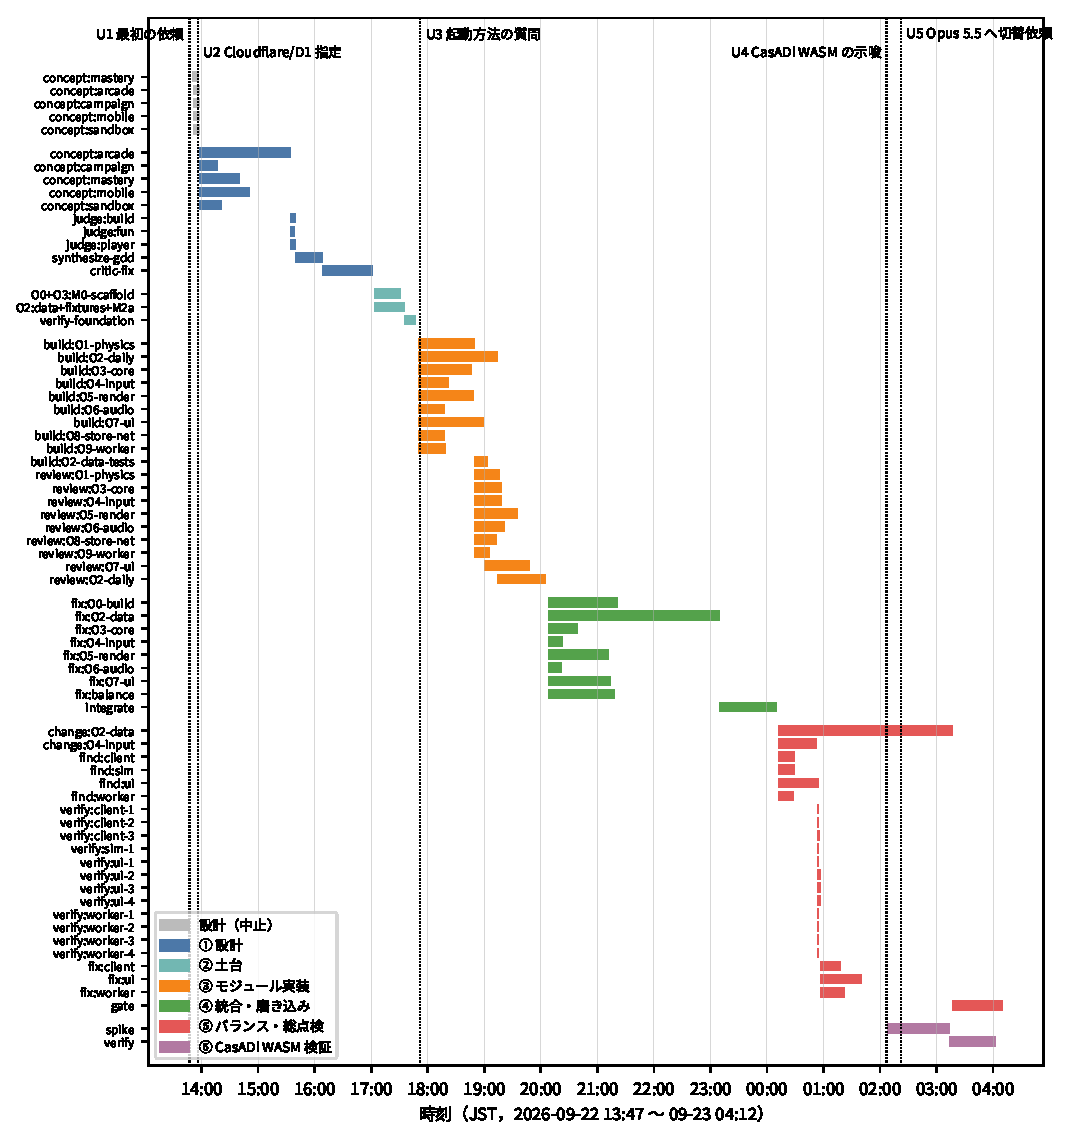
\includegraphics[width=\linewidth]{figs/gantt.pdf}
\caption{開発セッションにおけるサブエージェントの稼働時間．1行が1体．点線 U1〜U5 は人の発言（\tabref{tab:human}の H1〜H5）．
灰色の短い行は，H2 を受けて中止した最初の設計ワークフロー．}
\label{fig:gantt}
\end{figure}

\begin{table}[H]
\centering
\caption{ワークフローごとの規模．時間は壁時計，トークンは実行記録に残る合計}
\label{tab:wf}
\small
\begin{tabular}{llrrrr}
\toprule
& ワークフロー（台本名） & エージェント & 時間 [分] & ツール呼び出し & トークン [万] \\
\midrule
－ & \code{pendulum-game-design}（中止） & 5 & 6.5 & 29 & 39 \\
① & \code{pendulum-game-design} & 10 & 183.0 & 330 & 208 \\
② & \code{yurapita-foundation} & 3 & 44.5 & 240 & 84 \\
③ & \code{yurapita-modules} & 19 & 134.9 & 2,351 & 784 \\
④ & \code{yurapita-integrate-polish} & 9 & 241.7 & 1,399 & 332 \\
⑤ & \code{yurapita-balance-review} & 22 & 238.1 & 1,211 & 404 \\
⑥ & \code{casadi-wasm-spike} & 2 & 114.6 & 361 & 59 \\
\midrule
& 合計 & 70 & & 5,921 & 1,912 \\
\bottomrule
\end{tabular}
\end{table}

\begin{figure}[H]
\centering
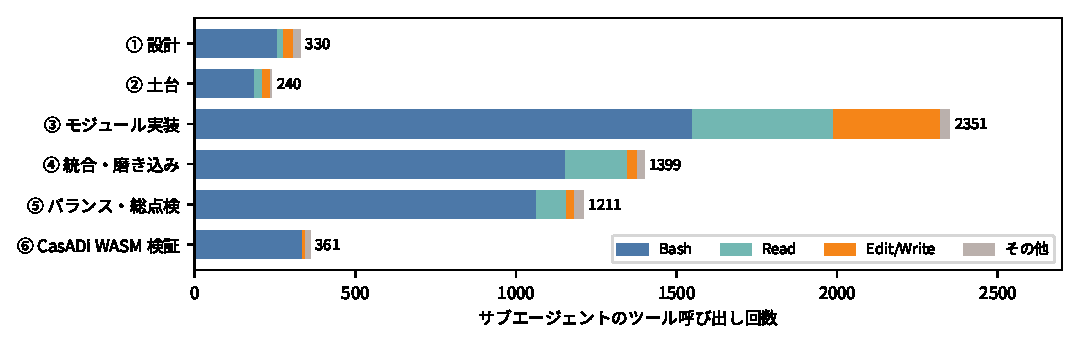
\includegraphics[width=\linewidth]{figs/toolmix.pdf}
\caption{ワークフローごとのツール呼び出しの内訳．ほとんどが Bash（テスト，ビルド，シミュレーション，スクリーンショット撮影）で，
「読んで書く」より「動かして確かめる」に手数を使っている．}
\label{fig:toolmix}
\end{figure}

工程は次の順に進んだ．各段の詳細は\secref{sec:phases}で述べる．
\begin{enumerate}
  \item[①] \textbf{設計}：5つの方向からゲーム案を出し，3人の審査役が採点し，1つの設計書にまとめ，抜けを直す．
  \item[②] \textbf{土台}：npm プロジェクト，モジュール間の型（契約），全ファイルの仮実装，面データ，仮の AI ゴーストを作る．
  \item[③] \textbf{並列実装}：9つのモジュールを担当エージェントが同時に作り，それぞれ別のエージェントがレビューして直す．
  \item[④] \textbf{統合と磨き込み}：モジュール間の依頼を片付け，人間らしいボットで難易度を調べ，全体を通しで確かめる．
  \item[⑤] \textbf{バランス調整と公開前の総点検}：難易度を直し，4つの観点で粗探し→反証→修正を行う．
  \item[⑥] \textbf{実現性の検証}：人のヒント（H4）を受けて，CasADi の WebAssembly 版がブラウザで使えるかを調べる．
\end{enumerate}
これに続いて，モデルの切り替えのための引き継ぎ，人の試遊を受けた調整，公開，宣伝動画の作成があった（\secref{sec:human}）．

\section{各工程とプロンプト}
\label{sec:phases}

\subsection{① 設計：独立した5案，3つの観点の審査，統合，批評}

指揮役は最初に研究コードの README と物理モジュールを読み，Node とブラウザとコア数を確かめてから，設計ワークフローを書いた．
全エージェントに共通の前置き \code{CONTEXT} には，運動方程式，壁の寸法，最適化器の性能，公開の条件がすべて数値で書かれている（\lstref{lst:context}）．

\begin{lstlisting}[caption={全エージェント共通の前置き（抜粋）},label={lst:context}]
It simulates a gantry crane: a trolley (mass M=2.0 kg) on a horizontal rail at height rail_y=1.25 m, a ball
(m=1.0 kg, radius 0.06 m) hanging on a massless inextensible STRING of length L=1.0 m. Input = horizontal force F
on the trolley (|F|<=40 N) ...
  (M+m) x'' + m L cos(th) th'' - m L w^2 sin(th) = F - b v
...
- Cheating: a public leaderboard will be attacked. Consider server-side verification: the Worker re-simulates a
  submitted per-tick input log with the SAME TypeScript physics module ... This needs bit-exact cross-engine
  determinism (fixed timestep, inputs quantized per tick, own sin/cos implemented with + - * / only because
  Math.sin differs between V8/JavaScriptCore/SpiderMonkey) and must fit the 10 ms CPU budget ...
- Scope: built by a team of AI coding agents in one session ..., so prefer depth and polish over sprawling
  feature lists. Must be genuinely fun, not a tech demo.
\end{lstlisting}
\begin{yaku}
これはガントリークレーンのシミュレーションである．水平のレール（高さ rail\_y = 1.25 m）の上を台車（質量 M = 2.0 kg）が走り，
長さ L = 1.0 m の質量のない伸びない\textbf{紐}でボール（m = 1.0 kg，半径 0.06 m）を吊っている．入力は台車に掛ける水平の力 F（$|F| \le 40$ N）である．…\\
$(M+m)\ddot{x} + mL\cos\theta\,\ddot{\theta} - mL\omega^2\sin\theta = F - bv$\\
…\\
・不正：公開ランキングは攻撃される．サーバー側での検証を検討すること．Worker は，送られてきたティックごとの入力の記録を\textbf{同じ} TypeScript の物理モジュールで再シミュレーションする．
これにはエンジンをまたいだビット単位の決定性が要る（固定の時間刻み，入力はティックごとに量子化，Math.sin は V8・JavaScriptCore・SpiderMonkey で結果が違うので sin/cos は + − × ÷ だけで自前実装する）．
さらに CPU 10 ms の予算に収めること．…\\
・規模：1セッションで AI のコーディングエージェントのチームが作る（…）．機能を広げるより，深さと磨き込みを優先すること．
技術デモではなく，本当に面白いものにすること．
\end{yaku}

最初の設計ワークフローは，公開先を claude.ai の Artifact と想定していた．
走り始めて9分後に H2（Cloudflare で公開，D1 を使ってよい）が届いたため，指揮役はワークフローを止め，
前置きの公開条件を Cloudflare の無料枠（1日 10 万要求，1要求 \SI{10}{ms} の CPU，D1 の読み書きの上限）と
サーバー側の再シミュレーションによる不正対策に書き換えて，やり直した．
\lstref{lst:context}の後半はこのとき足された文である．

\paragraph{5つの案} 5体のエージェントに，それぞれ別の方向からゲーム案を1つずつ作らせた（\tabref{tab:concepts}）．
方向の指示は1〜2文で，参考作品の名前を挙げて具体的にしている．たとえば mastery には
``\textit{The headline hook is `can a human beat the optimal-control AI?'}''（訳：「一番の売りは「人間は最適制御 AI に勝てるか？」である」），
mobile には ``\textit{The first 10 seconds must be self-explanatory without text}''（訳：「最初の 10 秒は文章なしでわかるものにすること」） と指示した．
出力は JSON スキーマで固定し，面の寸法をメートル単位で 12〜20 面ぶん書かせた．
案を作るエージェントの多くは，研究コードの最適化器や自作のシミュレーションを実際に動かして，面が解けるかを確かめていた
（arcade 案のエージェントは 96 分，38 回の Bash を使った）．

\begin{table}[H]
\centering
\caption{5つの案と審査の結果．点数は3人の審査役の重み付き合計（楽しさ×2，最初の1分×1.5，作りやすさ×1.5，独自性，研究への忠実さ）}
\label{tab:concepts}
\small
\begin{tabular}{llllr}
\toprule
方向 & 案の名前 & タグライン（抜粋） & 面数 & 合計点 \\
\midrule
mastery & ゆらしてピタッ & 最適制御AIに，人間の指で勝て． & 19 & \textbf{169.8} \\
mobile & フリピタ & 振って，越えて，ピタッと止めろ． & 16 & 158.0 \\
arcade & スレスレ・クレーン & 壁まで，あと3ミリ． & 18 & 152.0 \\
campaign & ユラピタ ―振り子クレーン― & ゆらして，越えて，ぴたっと止める． & 18 & 137.0 \\
sandbox & ふりこパーキング & 押せるのは台車だけ． & 20 & 128.8 \\
\bottomrule
\end{tabular}
\end{table}

\paragraph{3つの観点の審査} 審査役は「任天堂やインディーの感覚をもつ試遊責任者（楽しさ）」
「three.js，WebAudio，Cloudflare，決定的な物理を担う主任エンジニア（作りやすさ）」
「X でリンクを見てスマホで開き，30 秒しか我慢しない日本の技術者（プレイヤー）」の3人である．
3人とも mastery を土台に選んだ．それぞれが他の案から「移植すべき案」と「捨てるべき案」を挙げた．
移植されたのは，縦画面の下半分を操作盤にする相対ドラッグ（arcade），Wordle 風の共有文つきの「今日の5球」（mobile），
自動生成の表示名（mobile），壁との隙間を mm で見せる演出と「論文ライン」20 mm（arcade），
振り子の折り返しで振れ幅に応じた音程の拍子木が鳴る音（campaign）などである．
一方で，紐が壁の角に巻きつく物理や面エディタ（sandbox），点数・コンボの経済（arcade），
そして\textbf{指を離すと LQR の自動制御が揺れを止める仕組み（mobile）}を中心に据えることは，3人がそろって退けた．
理由は「題名の動詞である『ピタッ』をプレイヤーから取り上げる」「『人間の指で最適制御AIに勝て』と矛盾する」で，
残すとしてもランキング対象外の補助に留める，という判断だった．
この項目は\secref{sec:human}で，人の試遊によって形を変えて復活する．

\paragraph{統合と批評} 統合役には「別々の AI エンジニアが互いに話さずに並行して作れるほど正確に」書くよう求め，
12 章の必須項目（物理仕様，面の表，データ型，API と SQL，無料枠の計算，モジュールごとの所有ファイル，受け入れ基準つきのマイルストーン）を列挙した．
できた設計書 \code{GAME\_DESIGN.md} は約 2,300 行になった．

続く批評役には，``\textit{the lead engineer who must start building tomorrow}''（訳：「明日から作り始めなければならない主任エンジニア」） の立場で，
矛盾や解けない面を探し，設計書を直接直すよう指示した．
批評役は 53 分・177 回のツール呼び出しを使い，最適化器と自作のサーボ・シミュレーションを実際に走らせて，
次のような問題を見つけて直した．
\begin{itemize}
  \item 3面の制限時間が再現できなかった（1-3 の 3.0 秒は 13 分たっても解けず，4-1 の 4.0 秒は実行不能）．確認できた値に直した．
  \item 「一度ダッシュすると $64^\circ$ に届く」という演出の前提は，紐のたるみを入れた本来のモデルでは $61.9^\circ$ だった．
  \item 送信のまとめ方が D1 無料枠の「1回 50 文まで」と「本文 16 KB まで」を超えていた．
  \item 長い走行はサーバーの検証予算を常に超え，ランキングに永久に載らなかった．
  \item 人間が AI に勝てる余地（最適解より何\%速く解けるか）を各面で測る検査を追加した．
\end{itemize}

\subsection{② 土台：契約と仮実装を先に作る}

設計書を読んだ指揮役は，いきなり並列実装に入らず，2体を並べて土台を作らせた．
1体目は npm プロジェクト一式，設定，テストの枠組み（Node，3ブラウザ，Cloudflare の workerd，E2E）と，
\textbf{全ソースファイルの型つき仮実装}を作った．中身は \code{throw new Error('not implemented')} でよいが，
プロジェクト全体が型チェックを通る状態にする．
また，物理モジュールで \code{Math.sin} を使うと lint とテストが落ちることを，実際に置いて確かめるよう指示している．
2体目は Python 側で 18 面のデータ，研究コードと照合するためのテスト用データ，
それに\textbf{二分探索を省いた仮の AI ゴースト}（M2a）を作った．本番のゴーストは 1〜2 時間かかるので，他の担当を待たせないためである．
最後に3体目が，報告を鵜呑みにせずに全コマンドを自分で実行して検証した．

土台が終わると，指揮役は本番の AI ゴースト計算（全面で最短時間を二分探索）を 12 コアで裏に流し，
その間に並列実装を始めた．計算は 84 分で終わり，たとえば 3-1「非力モーター」の AI のタイムは仮の 13.9 秒から 5.57 秒になった．

\subsection{③ 並列実装：ファイル所有権と独立レビュー}

実装は，物理コア，ゲーム進行，入力，描画，音，UI，保存と通信，Worker と D1，日替わりの面の生成の9モジュールに分け，
担当 O1〜O9 に同時に作らせた．全員が同じ作業ツリーで動くので，共通の規則を細かく決めている（\lstref{lst:rules}）．

\begin{lstlisting}[caption={並列実装の共通規則（抜粋）},label={lst:rules}]
- Only create/modify files you own (listed in your task). Never edit other owners' files, never edit
  GAME_DESIGN.md ..., package.json, lockfile or shared configs. If you need a change elsewhere, write it in your
  report (requests_for_other_owners).
- Never run git commands that change state. Never run npm install. Do not touch anything outside game/.
- Other owners are implementing their stubs at the same time: code strictly against the contract types; when you
  need another module's behaviour in tests, use small fakes. ...
- If you run Playwright, ALWAYS set unique ports: PW_PREVIEW_PORT and PW_DEV_PORT env vars ...
- Quality bar: this must become a genuinely fun, polished game (Nintendo-level feel), not a tech demo. Verify your
  work by actually running it (tests, builds, screenshots you look at with the Read tool). Report failures honestly.
\end{lstlisting}
\begin{yaku}
・自分が所有するファイル（タスクに列挙したもの）だけを作成・変更すること．他の担当のファイル，GAME\_DESIGN.md（…），package.json，ロックファイル，共有の設定は決して編集しない．
ほかの場所の変更が必要なら，報告（requests\_for\_other\_owners）に書くこと．\\
・git の状態を変えるコマンドは決して実行しない．npm install も実行しない．game/ の外には触れない．\\
・ほかの担当も同時に自分の仮実装を実装している．契約の型に厳密に従ってコードを書くこと．テストで他のモジュールの振る舞いが必要なら，小さな偽物を使うこと．…\\
・Playwright を動かすときは\textbf{必ず}固有のポートを設定すること（環境変数 PW\_PREVIEW\_PORT と PW\_DEV\_PORT）．…\\
・品質の基準：技術デモではなく，本当に面白く，磨き込まれたゲーム（任天堂級の手触り）にすること．
実際に動かして確かめること（テスト，ビルド，Read ツールで自分の目で見るスクリーンショット）．失敗は正直に報告すること．
\end{yaku}

各担当のプロンプトには，所有ファイルの一覧，設計書の該当節，受け入れ基準が書かれている．
描画担当には ``\textit{LOOK at your screenshots with the Read tool and iterate until the scene is genuinely attractive and legible on a phone}''（訳：「スクリーンショットを Read ツールで見て，場面が本当に魅力的でスマホで読みやすくなるまで繰り返し直せ」），
UI 担当には ``\textit{Avoid generic `AI-looking' UI (no purple gradients, no glassmorphism)}''（訳：「ありがちな『AI っぽい』UI は避けること（紫のグラデーションもガラス風もなし）」） と，見た目の基準まで指定した．
物理担当には，研究コードとの誤差（1e-9），3ブラウザと workerd でのビット単位の一致，
5400 ステップを 5 ms 以内で計算できることを求めた．

台本は依存関係をそのまま表している（\lstref{lst:pipeline}）．
各モジュールは作り終えると，\textbf{物理コアの完成を待ってから}，別のエージェントのレビューに回る．
レビュー役は元の担当と同じファイルを所有し，``\textit{Adversarially review}''（訳：「敵対的にレビューせよ」） して直す．

\begin{lstlisting}[caption={作る→レビューする，の依存つきパイプライン（台本の抜粋）},label={lst:pipeline}]
const o1Build = agent(COMMON + ... + o1.task, { label: `build:${o1.key}`, phase: 'Build', schema: REPORT })
const o1Done = o1Build.then(r => r, () => null)
const reviewOf = async (m, build) => {
  await o1Done   // real integration with src/sim is possible only after the physics core is done
  return agent(COMMON + REVIEW_TASK(m, build), { label: `review:${m.key}`, phase: 'Review', schema: REPORT })
}
\end{lstlisting}
\begin{yaku}
（コード中のコメントの訳）物理コアが完成して初めて，src/sim との本当の統合ができる．
\end{yaku}

レビューは形だけでは終わらなかった．\tabref{tab:review}に主な発見を示す．
いずれも作った本人が「受け入れ基準はすべて通過」と報告したあとに見つかったものである．

\begin{table}[H]
\centering
\caption{独立レビューで見つかった主な不具合（③）}
\label{tab:review}
\small
\begin{tabularx}{\linewidth}{lX}
\toprule
モジュール & 発見（重大度） \\
\midrule
物理 & レール端で台車が止まっているとき，ボールが振れの途中で空中に止まる（高）．
「GC ゼロ」の主張が誤りで，最適化後のコードは1ステップ 32 バイトを確保していた（中） \\
ゲーム進行 & 振れ幅メーターなど，ボールに付いて動く表示が本番の画面に一つも出ていなかった．スマホを回すと目標位置が消えた（高） \\
描画 & NaN が1回入ると時計とカメラが壊れ，次の開始まで画面が真っ白になる（高） \\
音 & 失敗を知らせる衝突音が，振り子の拍子音より 6〜9 dB 小さく，しかもスマホのスピーカーで鳴らない低域に偏っていた（高） \\
UI & NaN が「NaN mm」とそのまま表示された．練習走行にも「自己ベスト更新」が出た（高） \\
保存と通信 & 2つ目のタブを閉じると，もう一方のタブで保存した進行が消える．3ブラウザで再現（高） \\
Worker & 仕様の誤りはないが，テストが報告より弱く，分の境目をまたぐと失敗する不安定なテストがあった（中） \\
\bottomrule
\end{tabularx}
\end{table}

\subsection{④ 統合と磨き込み：決定事項，難易度調査，通しプレイ}

③の結果を読んだ指揮役は，自分で開発サーバーを立ててスクリーンショットを2枚見たうえで，
各担当の「他の担当への依頼」と「設計からの逸脱」を裁定し，\textbf{決定事項 D1〜D10} として次の台本の冒頭に書いた
（``\textit{LEAD DECISIONS (binding; they override the spec where they differ)}''（訳：「指揮役の決定事項（拘束力あり．仕様と食い違う場合はこちらが優先）」））．
たとえば D10 は，縦画面の上 4 割が空白の紙になっていることを指摘し，カメラの追従幅とスコア表示の配置を担当2人に分けて直させた．

同じワークフローで，\textbf{人間らしい操作をするボット}による難易度調査も並行させた．
指示は具体的で，タッチは「折れ点 6 個以下，間隔 0.15 秒以上，目標速度 \SI{5}{m/s} 以下の折れ線」，
キーボードは「切り替え 7 回以下，間隔 0.12 秒以上」とし，
最良の操作に時刻 $\sigma = 40$ ms，位置 $\sigma = 1$ cm のぶれを加えて 50 回ずつ成功率を測るよう求めた．
エージェントは交差エントロピー法で操作を最適化し，本物のシミュレーター・サーボ・入力処理を使って 18 面と日替わり 12 面を調べた．
結果，4-3「たまご」は銅メダルが取れない，5-2 は銅メダルでも 9\%，キーボードでは 2-2 を一度もクリアできない，
日替わりの AI のタイムは甘すぎる，といったことがわかった．

最後に統合役が全ファイルの所有権を引き継ぎ，全テストを通したうえで，
390×844 のタッチと 1280×720 のマウスで，実際の操作による通しプレイを撮影して確かめた．
スクリーンショットから，結果カードの上のボタンが押せない，320 px 幅でボタンの文字が1文字ずつ折れる，など 10 件を見つけて直した．

\subsection{⑤ バランス調整と公開前の総点検：粗探し→反証→修正}

指揮役は難易度調査の結果から，5-2 の奥の壁を 5 cm ずらす，たまごの割れる張力を 16 N から 18 N に上げる，
キーボードを「短く押すと 5 cm 動く」ようにする，日替わり 84 面の AI のタイムを 0.1 秒刻みで解き直す，と決めた．
これと並行して，公開前の総点検を次の3段で行った（\lstref{lst:review}）．

\begin{enumerate}
  \item \textbf{粗探し}：サーバー（攻撃者と急な人気集中の視点），物理（再生と不正対策の一致），ゲーム進行，見た目と音の4観点で，
  読み取り専用のエージェントが不具合を探す．「具体的な失敗の筋書きがないものは書くな」と指示した．
  \item \textbf{反証}：中・高の指摘1件ごとに，別のエージェントが反証を試みる．``\textit{Default to real=false if you cannot substantiate it}''（訳：「裏付けられなければ real=false とせよ」）．
  \item \textbf{修正}：観点ごとに1体が，確定した指摘を直し，1件ごとに回帰テストを足す．
\end{enumerate}

\begin{lstlisting}[caption={反証役へのプロンプト（全文）},label={lst:review}]
# Role: skeptical verifier (read-only on the game source; scratch under /tmp/claude-1000/yp-verify/${f.id}/).
Try to REFUTE this finding. Read the code paths involved, and if cheap, reproduce it with a small script/test.
Default to real=false if you cannot substantiate it. If real, give the right severity and the best fix.
Finding: ${JSON.stringify(f)}
\end{lstlisting}
\begin{yaku}
\# 役割：懐疑的な検証役（ゲームのソースは読み取り専用．作業用のファイルは /tmp/claude-1000/yp-verify/\$\{f.id\}/ に置く）．\\
この指摘を\textbf{反証}せよ．関係するコードの経路を読み，手間が小さければ小さなスクリプトやテストで再現すること．
裏付けられなければ real=false とすること．本物なら，正しい重大度と最善の修正を示すこと．\\
指摘：\$\{JSON.stringify(f)\}
\end{yaku}

指摘は 26 件（高 3，中 9，低 14）出た．中・高の 12 件はすべて反証に耐えたが，高とされた3件はすべて「中」に下げられた．
主なものを\tabref{tab:findings}に示す．修正役は，回帰テストが元のコードで本当に落ちることも確かめている
（サーバーの回帰テスト 20 件のうち 16 件が元のコードで失敗した）．

\begin{table}[H]
\centering
\caption{公開前の総点検で確定した指摘（抜粋）}
\label{tab:findings}
\small
\begin{tabularx}{\linewidth}{lX}
\toprule
観点 & 指摘 \\
\midrule
サーバー & 他人の公開リプレイを，新しい秘密鍵で何度でも送り直してランキング上位 100 を埋められる \\
サーバー & IPv6 では同じ /64 から無制限に送れる（回数制限のキーが完全なアドレス） \\
サーバー & 別サイトからの単純な POST（text/plain）を受け付けてしまう \\
進行 & 日替わりの5球目の最中に画面を隠すと，その球の結果が送られない \\
進行 & 日替わりの起点日が公開日より後のままだと，再訪した人の日替わりが止まる \\
見た目 & 王冠や自己ベストの帯が結果カードの裏に描かれ，見えない \\
見た目 & 320〜375 px の画面で，結果ボタンの文字が単語の途中で折れたり1文字に切れたりする \\
\bottomrule
\end{tabularx}
\end{table}

最後のゲート役は，全テスト（単体 1,299，ブラウザ 80，E2E 262）を通し，難易度を測り直した．
たまごの銅メダル到達率は 0\% から 32\% に，5-2 は 9\% から 35\% になった．
ただしキーボードで 2-2 をクリアできる率は 0.2\% から 1.0\% にしか上がらず，
ゲート役は「キーボードの失敗の 8〜9 割は最後の止め方ではなく壁への衝突」と原因を正しく報告している．
この弱点は，人の試遊で指摘されるまで残った．

\subsection{⑥ 実現性の検証：CasADi WebAssembly}

⑤の最中に，人が「CasADi 3.8.1 が js/WebAssembly に対応しているから，必要に応じて使ってね」と伝えた（H4）．
指揮役はすぐに組み込まず，ゲームのファイルに触れない場所で試す2体のワークフローを立てた．
1体目は研究の最適化問題を JS に移し，Python と目的関数がビット単位で一致すること，
ブラウザの Web Worker で動き，既存の解から始めれば 0.4〜0.5 秒で解き直せることを示した．
2体目はその数値を測り直すとともに，配布されている IPOPT のプラグインに METIS 4 の関数が 39 個含まれ，
そのライセンスが無許可の再配布を禁じていることを見つけた．
指揮役はこの結果から「いまは使わない．METIS を外した版か，定式化を変えて fatrop を使えるようになったら，
失敗した瞬間から AI が解き直す機能を入れる」と決め，引き継ぎメモに残した．

\subsection{引き継ぎ：モデルの切り替え}

人が「キリがついたら Opus 5.5 で続けて」と依頼した（H5）とき，裏で2本のワークフローが動いていた．
指揮役はこの依頼をタスクキューに積み，両方が終わるのを待ってから，
現状，決定事項，残作業，公開手順，注意点をまとめた \code{game/docs/HANDOFF.md} を書き，
自分の記憶ファイルからもそこを指すようにしたうえで，再起動を依頼した．
新しいセッションは「HANDOFF.md を読んで続きをやって」の一言で作業を再開し，
残っていた細かい表示の不具合を直した．

\section{面白さの評価}
\label{sec:fun}

依頼の核は「最強に面白いゲーム」だったが，公開前に人が遊んだのは H7 の1回だけである．
では，エージェントたちは面白さを何で測っていたのか．記録を読むと，評価は次の5段に分かれていた．
\begin{enumerate}
  \item \textbf{案を作る段}：各案に「なぜ最も面白いか」と「最初の 60 秒」を書かせる（自己申告）．
  \item \textbf{審査の段}：3人の審査役が5つの軸で 0〜10 点を付け，重みを付けて合計する（\secref{sec:fun-judge}）．
  \item \textbf{設計書の段}：面白さを「名前の付く技」「最初の 60 秒の秒単位の台本」に分解して書き下す（\secref{sec:fun-gdd}）．
  \item \textbf{実装の段}：「任天堂級の手触り」を品質基準として全員に課し，スクリーンショットを見て判断させる（\secref{sec:design}）．
  \item \textbf{数値の段}：人間らしいボットでメダルの取りやすさを測る（\secref{sec:phases} ④⑤）．
\end{enumerate}
このうち点数が付いたのは2段目だけで，数値で測ったのは5段目の「難しさ」だけである．
「遊んで面白いか」を直接確かめた工程は，人の試遊（\secref{sec:human}）までなかった．

\subsection{審査の軸と重み}
\label{sec:fun-judge}

審査役の出力は JSON スキーマで固定されていた（\lstref{lst:judgeschema}）．
面白さに関わる軸は2つで，``\textit{moment-to-moment fun and replayability}''（訳：「その瞬間瞬間の楽しさと，繰り返し遊びたくなるか」）（楽しさ）と
``\textit{how quickly a newcomer gets it and gets hooked}''（訳：「初めての人がどれだけ早く理解し，はまるか」）（最初の1分）である．
これに作りやすさ，独自性，研究への忠実さを加えた5軸を，台本の中で次の式で合計した．
\begin{lstlisting}[caption={重み付き合計（台本の抜粋）},label={lst:weight}]
for (const j of judged) for (const s of j.scores) {
  const t = s.fun * 2 + s.first_minute * 1.5 + s.feasibility * 1.5 + s.originality + s.fidelity
\end{lstlisting}
重みは指揮役が台本を書いた時点で決めたもので，楽しさを2倍にしている．
審査役にはこの重みを知らせていない．点数とは別に，土台にする案（\code{recommended\_base}），
移植すべき案と捨てるべき案，操作方式と失敗条件についての判定も書かせた．

3人の審査役の観点（\secref{sec:phases} ①）のうち，「楽しさ」の観点のプロンプトは次のとおりである．
\begin{lstlisting}[caption={審査役「楽しさ」の観点（全文）},label={lst:funlens}]
You are a veteran game designer and playtest lead (Nintendo EPD / indie hit sensibility). Judge primarily on
fun, game feel, pacing, difficulty curve, retention and "one more try" pull. Be harsh on frustration, filler
levels and features that dilute the core.
\end{lstlisting}
\begin{yaku}
あなたはベテランのゲームデザイナーで，試遊の責任者である（任天堂 EPD やヒットしたインディーの感覚をもつ）．
主に，楽しさ，手触り，テンポ，難易度曲線，継続して遊びたくなるか，「もう一回」の引力で評価せよ．
イライラさせるもの，埋め草の面，コアを薄める機能には厳しくすること．
\end{yaku}

\tabref{tab:judgeaxes}に，軸ごとの点数（3人の合計，各 30 点満点）を示す．

\begin{table}[H]
\centering
\caption{審査の軸ごとの点数（3人の審査役の合計．各軸 30 点満点）と重み付き合計}
\label{tab:judgeaxes}
\small
\begin{tabular}{lrrrrrr}
\toprule
案 & 楽しさ & 最初の1分 & 作りやすさ & 独自性 & 忠実さ & 重み付き合計 \\
 & ($\times2$) & ($\times1.5$) & ($\times1.5$) & ($\times1$) & ($\times1$) & \\
\midrule
mastery & 24.5 & 24.0 & \textbf{23.5} & 20.5 & \textbf{29.0} & \textbf{169.8} \\
mobile & 21.5 & \textbf{27.0} & 20.0 & 20.5 & 24.0 & 158.0 \\
arcade & \textbf{25.0} & 24.0 & 15.0 & 22.5 & 21.0 & 152.0 \\
campaign & 21.5 & 17.5 & 12.5 & 25.5 & 23.5 & 137.0 \\
sandbox & 22.0 & 21.0 & 7.5 & \textbf{27.0} & 15.0 & 128.8 \\
\bottomrule
\end{tabular}
\end{table}

表から次のことが読み取れる．
\begin{itemize}
  \item \textbf{楽しさの軸だけなら arcade が1位だった}．「楽しさ」の審査役と主任エンジニアの2人が arcade に最高点（8.5）を付け，
  楽しさの合計は arcade 25.0，mastery 24.5 と僅差だった．
  arcade を2位以下に落としたのは作りやすさ（15.0 対 23.5）で，点数の経済（ニアミスの段階×コンボ×収集物）が
  「1セッションで磨き上げられるか」の点で割り引かれた．
  \item \textbf{楽しさの軸は差がつきにくかった}．5案の合計は 21.5〜25.0 に収まり，幅は 3.5 点しかない．
  一方，作りやすさは 7.5〜23.5 と大きく開いた．結果として，順位を最も大きく動かしたのは作りやすさだった．
  \item \textbf{最初の1分は mobile が3人とも 9 点}だった．文章なしの導入と「今日の5球」は，土台に選ばれなかった mobile 案から移植された．
\end{itemize}

審査役のコメントも，面白さを抽象語ではなく仕組みで語っている．
「楽しさ」の審査役は mastery を「5案で最も強いコアループ．カウントダウンがなく，最初の入力で時計が動き，リトライは 100 ms 未満，壁ごとにスプリットが出る Trackmania 型」と評した．
sandbox には「壁に触れても無害にすると，他の案すべてが頼っている『ミリ単位の緊張』が消える．AI の 2 cm の余裕に意味がなくなる」と書いた．
「プレイヤー」の審査役は mastery の「AI のルールを破ることで AI を超える」という筋を「正直で，とても投稿したくなる」と評価している．
つまり審査役たちは，面白さを「緊張（壁 0 mm）」「即リトライ」「比べられる相手（AI）」「語れる物語」の組み合わせとして捉えていた．

\subsection{設計書での面白さの言語化}
\label{sec:fun-gdd}

統合役への指示には，設計書の第1章として ``\textit{what makes it 最強に面白い}''（訳：「何がこれを最強に面白くするのか」），
第2章として ``\textit{the first 60 seconds (moment by moment; no text walls - teach by play)}''（訳：「最初の 60 秒（瞬間ごとに．文章の壁は置かず，遊びで教える）」） を必須にしていた．
その結果，設計書は面白さを次の3つの粒度で書き下している．
\begin{itemize}
  \item \textbf{柱（3本）}：「人類 vs 最適制御」「ミリで攻めて，ピタッで決める」「一瞬でもう一回」．
  AI は壁から 2 cm 離れ，紐の張力を保つ．人間は壁 0 mm まで攻めてよく，紐をたるませてもよい．
  「AI に勝つ方法は，この自由を使うことだけ」と，勝ち筋そのものを物理の規則の差として設計している．
  \item \textbf{名前の付く技}：遅れ，ブレーキ振り出し，逆振りの溜め，共振ポンプ，追いかけ減衰，端ドン，パシッの7つ．
  入力は台車の目標位置1つだけだが，劣駆動の振り子なので技が自然に生まれる，という主張である．
  技を見つけると技名のトーストが出て，「自分で発見した」感覚を残す．
  \item \textbf{最初の 60 秒の台本}：0:00 から 0:58 まで，何秒に何が起き，プレイヤーが何を感じるかを表にしている
  （例：「0:27 最初のクラッシュ．ゴンッ，レンガが飛び，0.08 秒のヒットストップ，接触点の赤丸と『−4 mm』」→「最初のクラッシュが笑える」，
  「0:42 すれすれで越える．スローモー，寸法線つきの『ギリ 9mm』」→「自慢の数字が出る」）．
\end{itemize}
面白さの主張が，このように検証可能な仕組み（リトライ 100 ms 未満，ヒントの開く回数，演出の秒数）に落ちていたため，
後の工程ではそれぞれを受け入れ基準や E2E テストとして確かめられた．
一方で，「この台本どおりに人が感じるか」は，どの工程でも確かめていない．

\section{ユーザー体験の分析}
\label{sec:ux}

\tabref{tab:ux}に，ユーザー体験に関わる主な決定を，その由来と確かめ方とともにまとめる．
由来の多くは①の審査で他の案から移植されたもので，確かめ方の多くは E2E テストかスクリーンショットだった．

\begin{table}[H]
\centering
\caption{ユーザー体験に関わる主な決定．由来は，その考えが最初に出た案または工程}
\label{tab:ux}
\small
\begin{tabularx}{\linewidth}{l>{\raggedright\arraybackslash}X>{\raggedright\arraybackslash}p{0.16\linewidth}>{\raggedright\arraybackslash}p{0.2\linewidth}}
\toprule
場面 & 決定 & 由来 & 確かめ方 \\
\midrule
導入 & タイトルからメニューを挟まず 1-1 が始まる．文章は出さず，半透明の手が操作を見せる．時計は最初の入力で動く & mobile & E2E，通しプレイ \\
導入 & 失敗 3・6・10 回でヒントを1行ずつ開く．未クリアの面で3連続クラッシュすると AI の手本を 0.5 倍速で1回だけ自動再生 & mobile，mastery & core のテスト \\
操作 & 全デバイスで「目標位置→サーボ→量子化した力」の1本の経路．縦画面は下 38\% を操作盤にし，どこを触っても相対ドラッグ & arcade，審査 & 入力テスト（1 m 動かして行き過ぎ 7 cm 以下） \\
操作 & 力バーに AI の同時刻の力を重ね，目標と台車を結ぶばね線を飽和で赤くする & mastery，sandbox & 描画のスクショ \\
失敗 & 壁は即クラッシュ，紐のたるみとレール端は物理として続行．0.7 秒の演出の間も入力すればすぐ戻る．リトライ 100 ms 未満 & 審査（3人一致） & E2E（READY まで 100 ms 未満） \\
失敗 & クラッシュ地点に赤丸と「−4 mm」，壁に直近5回の赤い×を残す & campaign，arcade & 描画のスクショ \\
報酬 & ニアミスを点数でなく mm の数字と寸法線で見せる．20 mm の「論文ライン」 & arcade（点数経済は削除） & UI のスクショ \\
社会 & 今日の5球，Wordle 風の共有行，挑戦状リンク，自動生成の表示名 & mobile & E2E（リンクの往復） \\
環境 & オフラインでも遊べ，API が落ちても「オフライン」の札を出すだけ & 設計書 & E2E（\code{/api/*} を遮断） \\
配慮 & 揺れ・フラッシュを OS の reduced motion に従わせる．文字 125\%．タッチ目標 44 px 以上．ゴーストは色に加えて形とラベルで区別．音だけの合図には見える対を付ける & 設計書 \S 3.5 & UI の E2E（44 px を全画面で検査） \\
\bottomrule
\end{tabularx}
\end{table}

\paragraph{審査が UX を決めた例：操作方式} 審査スキーマには点数と別に \code{control\_scheme\_verdict} を設けていた．
3人は独立に「全デバイスで1つのサーボ経路を出荷し，同じ手触りと同じランキングを共有する」と判定した．
「プレイヤー」の審査役はサーボの固有振動数を振り子の2倍（約 6.5 rad/s），減衰比を約 0.8 にし，
「台車は正確に感じるが瞬間移動はできず，ボールがはっきり遅れる」ように決めている．
一方，campaign 案と sandbox 案の「力を直接指定し，離すと惰性で進む」操作は，3人とも既定の操作から外した．

\paragraph{UX の不具合はどこで見つかったか} 作った本人が見落とし，別のエージェントが見つけた UX の問題は多い．
UI のレビュー役は約 20 件を直した．たとえば，ポーズメニューのゴースト切り替えの表示が実際の状態を推測で描いていた，
「NaN mm」がそのまま共有カードに載った，などである．
統合役は実際のタッチ操作で通しプレイし，10 件を直した．
公開前の総点検では，UI 観点の粗探し役に次の観点を与えている（抜粋）．
\begin{lstlisting}[caption={総点検の UI 観点（抜粋）},label={lst:uifind}]
UI/UX, rendering and audio quality: ... Look for layout overlap/clipping at 320-430 px portrait and landscape
phones and desktop, text overflow in ja and en, focus traps, keyboard operability, touch targets < 44 px, safe
areas, reduced motion, i18n gaps ..., wrong numbers/formatting (NaN, Infinity, negative), memory leaks ...,
and anything that would look broken in a screenshot shared on X.
\end{lstlisting}
\begin{yaku}
UI/UX，描画，音の品質：…
320〜430 px の縦持ち・横持ちのスマホとデスクトップでのレイアウトの重なりやはみ出し，日本語と英語での文字のあふれ，フォーカスの閉じ込め，キーボードで操作できるか，
44 px 未満のタッチ目標，セーフエリア，reduced motion，翻訳の抜け（…），数値や書式の誤り（NaN，Infinity，負の値），メモリリーク（…），
そして \textbf{X で共有されたスクリーンショットで壊れて見えるもの}すべてを探せ．
\end{yaku}
最後の ``\textit{anything that would look broken in a screenshot shared on X}''（訳：「X で共有されたスクリーンショットで壊れて見えるものすべて」） は，公開先の文脈を UX の基準にしたものである．
反証役もこの基準で重大度を判断しており，360 px 幅で「ランキング」の文字がカタカナの途中で折れる不具合を
「機能は壊れていないが，X でスクリーンショットを撮られる結果画面の見た目の傷」として中と判定した．

\paragraph{UX で届かなかったところ} ボットによる難易度調査は「キーボードでは 2-2 をほぼクリアできない」ことを数値で示したが，
入力の手触り（押した瞬間に最高速へ達する）を原因として特定し直すことはなかった．
これは人の試遊の「減衰させようとすると加速する」で初めて特定された（\secref{sec:human}）．
UX の検証が「画面が壊れていないか」には強く，「操作して気持ちよいか」には弱かったことを示している．

\section{デザインの分析}
\label{sec:design}

\subsection{方針：「工房の机の上のジオラマ × 実験ノート」}
設計書のアートディレクションは，研究の動画と同じ語彙（レンガ壁，ガントリー，赤いボール）に，
製図のインク線（寸法線，角度の弧，判子）を重ねるものである．
方針は審査役の案をもとに統合役が決め，各担当のプロンプトで繰り返し念を押している．
\begin{itemize}
  \item UI 担当：``\textit{Avoid generic `AI-looking' UI (no purple gradients, no glassmorphism): it should feel like a warm lab notebook / drafting card with bold rounded Japanese type.}''（訳：「ありがちな「AI っぽい」UI は避けること（紫のグラデーションもガラス風もなし）．太い丸ゴシックの日本語の文字で，温かい実験ノートや製図カードのように感じられること」）
  \item 描画担当：``\textit{a beautiful, warm "workbench diorama $\times$ lab notebook" three.js scene built only from primitives and canvas textures}''（訳：「プリミティブと canvas のテクスチャだけで組んだ，美しく温かい「工房のジオラマ × 実験ノート」の three.js の場面」）
  \item 音担当：``\textit{Make it sound GOOD: tasteful levels, no harshness, the apex ticks must feel musical (this replaces BGM).}''（訳：「良い音にせよ．品のよい音量で，耳障りな音はなし．折り返しの拍子音は音楽的に感じられること（これが BGM の代わりになる）」）
\end{itemize}

\paragraph{色と文字} 色は 21 個のトークンとして設計書に書かれ，CSS と three.js で同じ値を使う（\tabref{tab:palette}）．
紙（\#F3EEE4），墨（\#1E2A44），レンガ，ガントリーの黄色が地で，意味を持つ色（ゴールの緑，危険の赤，AI のシアン）は
着せ替えでも変えない約束になっている．
文字は丸ゴシック（M PLUS Rounded 1c の 800 と 500）で，数字は等幅にしてタイムが揺れないようにした．

\begin{table}[H]
\centering
\caption{色のトークン（抜粋，\code{GAME\_DESIGN.md} \S 9.1）}
\label{tab:palette}
\small
\begin{tabular}{lll}
\toprule
トークン & 値 & 用途 \\
\midrule
\code{--paper-1} / \code{--paper-2} & \#F3EEE4 / \#E6DCCB & 背景の紙 \\
\code{--ink} & \#1E2A44 & 製図線，寸法，UI の文字 \\
\code{--brick-1} / \code{--brick-2} & \#B5553A / \#C8643F & レンガ（1個ずつ色相を揺らす） \\
\code{--gantry} & \#F2B705 & ガントリーの梁 \\
\code{--ball} & \#E0312B & ボール \\
\code{--goal} & \#22B573 & ゴール，静止リング \\
\code{--danger} & \#E5484D & クラッシュ，飽和 \\
\code{--ai} & \#19C3FF & AI ゴースト（加算合成と走査線） \\
判子 & \#D8342B & 「ピタッ!」の朱色の判子 \\
\bottomrule
\end{tabular}
\end{table}

\paragraph{素材を持たない} 画像・モデル・音声のファイルは1つもない．
テクスチャは起動時に canvas で最大6枚を描き，モデルはプリミティブで組み，効果音はすべて WebAudio のレシピ（\tabref{tab:sound}）で合成する．
BGM は置かず，振り子の折り返しで鳴る拍子木の音を，振れ幅に応じて C メジャー・ペンタトニックの 15 段に割り当てた．
振るほど音程が上がり，共振ポンプがそのまま旋律になる．

\begin{table}[H]
\centering
\caption{効果音のレシピ（抜粋，\code{GAME\_DESIGN.md} \S 9.6）}
\label{tab:sound}
\small
\begin{tabularx}{\linewidth}{lX}
\toprule
音 & レシピ \\
\midrule
拍子木（折り返し） & 正弦波と 2.4 倍の正弦波，5 ms のノイズのクリック．振れ幅 0〜90° を C4〜C7 のペンタトニック 15 段に \\
ニアミス & 正弦 2.4→3.2 kHz のグライド 120 ms．すき間の区分ごとに1半音ずつ上げる \\
紐の張り直し & Karplus-Strong（遅延 1/220 s，減衰 0.996）．音量は撃力に比例 \\
静止保持と成功 & C5 D5 E5 G5 A5 の5段を 0.1 s ごと，成功で C–E–G の和音 \\
クラッシュ & 正弦 70→40 Hz，ローパスしたノイズ，レンガが崩れるクリック 8 回 \\
\bottomrule
\end{tabularx}
\end{table}

\paragraph{ジュース表} 設計書には，ゲーム内のイベント 18 種それぞれについて，見た目・音・振動を1行で決めた表がある．
たとえば成功は「リングが完成し 0.15 s 静止 → 判子を 1.6 倍から 1.0 倍へ 120 ms で押す → 軌跡が 0.1 s 刻みのストロボ点に固まる → 紙吹雪」
と長三和音，振動 20 ms である．演出の担当（描画・UI・音）が別々でも，同じ表を見て作れば1つの手触りに揃う．

\paragraph{性能予算} 見た目の質を性能と引き換えにしないよう，予算も数値で決めた（描画呼び出し 40 以下，三角形 6 万以下，
メイン JS は gzip で 450 KB 以下，中位のスマホで 60 fps）．統合時点の実測は，描画呼び出し 21〜23，メイン JS 315 KB だった．

\subsection{目で見て直す}
デザインの検証は，数値の検査よりもスクリーンショットを見ることで行われた．
開発セッションのサブエージェントが画像を読み込んだ回数は合計 559 回で，その大半は UI と描画の担当だった（\tabref{tab:shots}）．
指揮役自身も4回スクリーンショットを見ており，そこから D10（縦画面の上 4 割が空白）を出している．

\begin{table}[H]
\centering
\caption{スクリーンショットを読み込んだ回数（開発セッション，上位）}
\label{tab:shots}
\small
\begin{tabular}{lr@{\hspace{3em}}lr}
\toprule
エージェント & 回数 & エージェント & 回数 \\
\midrule
UI のレビュー役（③） & 91 & 描画のレビュー役（③） & 34 \\
UI の担当（③） & 72 & 描画の修正（④） & 33 \\
UI の修正（④） & 61 & UI の修正（⑤） & 28 \\
統合役（④） & 58 & 描画の担当（③） & 28 \\
UI の粗探し役（⑤） & 53 & 音の担当・レビュー・修正 & 18 \\
\midrule
\multicolumn{3}{l}{合計（全エージェント）} & 559 \\
\bottomrule
\end{tabular}
\end{table}

見ることで見つかった問題の例を挙げる．
\begin{itemize}
  \item 描画のレビュー役：縦画面で，実験ノート風の見出しが左端で切れ，さらに UI のロゴやボタンと重なっていた．
  設計書にあったクラッシュ時の赤いビネットが，描画と UI のどちらにも実装されていなかった．
  \item 指揮役：縦画面の 3D ビューの約 4 割が，ガントリーより上の空白の紙だった（→ D10．カメラの追従幅を 2.0〜2.3 m にし，空いた上部を AI・時計・自己ベストのスコアボードにした）．
  \item 統合役：結果カードの上のボタンがトーストに隠れて押せない．320 px 幅でボタンの文字が1文字ずつ折れる．
\end{itemize}

音も「聞く」代わりに測った．音のレビュー役は全効果音の A 特性の音量，スマホのスピーカーを模した 400 Hz のハイパス版，スペクトログラムを計算し，
失敗を知らせる衝突音が拍子木より 6〜9 dB 小さく，しかもスマホで鳴らない 40〜70 Hz に偏っていることを見つけた（\tabref{tab:review}）．
低域の正弦波を奇数倍音へ歪ませる「スマホ用の層」を足し，衝突音を拍子木より約 4 dB 大きくして直している．

\section{人の試遊と公開}
\label{sec:human}

\subsection{「難しすぎる」}

公開前に筆者が遊び，「難しすぎる．減衰させようとすると加速する．矢印キーだけだと微調整がしづらすぎる」と伝えた（H7）．
Opus 5.5 の指揮役はワークフローを使わず，自分で原因を調べて直した．
キーボードは「速度を操る」方式で，ちょっと押しただけで 0.17 秒で最高速に達するため，
止めようとして押すたびに揺れを大きくしていた．ボットの調査でもキーボードは 2-2 のクリア率が 1\% 未満だった．

指揮役は，ゴールの 30 cm 以内で手を離すと離散時間 LQR が揺れを止めてボールをゴールの内側へ寄せる
「ゆれ止めアシスト」を実装した．ゲイン候補の格子探索と閉ループのシミュレーションを本物の物理で行い，
止まるまでの時間はパッド面で 15〜24 秒から 2〜3.6 秒に，ポケット面で 7〜15 秒から 1.6〜1.9 秒に縮んだ．
記録されるのは台車に掛けた力の列だけなので，サーバーの再シミュレーションによる検証はそのまま使える．
あわせてキーボードの加速を半分にし，それに合わせて入力テスト 26 件の期待値を直す作業だけを，
「テストを骨抜きにしない」という条件つきでサブエージェント1体に任せた．

この変更は，①の審査で3人がそろって退けた「指を離すと LQR が揺れを止める」案（mobile 案）とほぼ同じものである．
審査役は「『ピタッ』をプレイヤーから取り上げる」として，ランキング対象外の補助に留めるよう求め，設計書でも優先度の最も低い P2 に置かれていた．
人が実際に遊ぶと，それがないと難しすぎた．結果として，この補助は既定でオン，ランキング対象で出荷された．

\subsection{公開}

公開の段階で，指揮役は外部に影響する操作を人に委ねた．
日替わりの起点日（公開後は変えられない）を選択肢で尋ね，
ビルドがまっさらな状態から通ることを確かめたうえでコミットと push を行い，
Cloudflare の画面での D1 の作成と GitHub リポジトリの接続は，手順を示して人にやってもらった．
これは筆者が「自分でリポジトリを選ぶところをやってみたい」と頼んだためでもある．
公開は 2026-09-23 11:59 JST だった．

その後，宣伝動画を依頼した（H10）．指揮役はゲームのテスト用フックを使って本物のタッチ操作を録画し，
シミュレーターで「ちゃんとクリアできる指の動かし方」を先に探してから撮影した．
ナレーションは VOICEVOX（ずんだもん），編集は Remotion で，27.6 秒の縦動画になった．

\begin{figure}[H]
\centering
\begin{subfigure}{0.24\linewidth}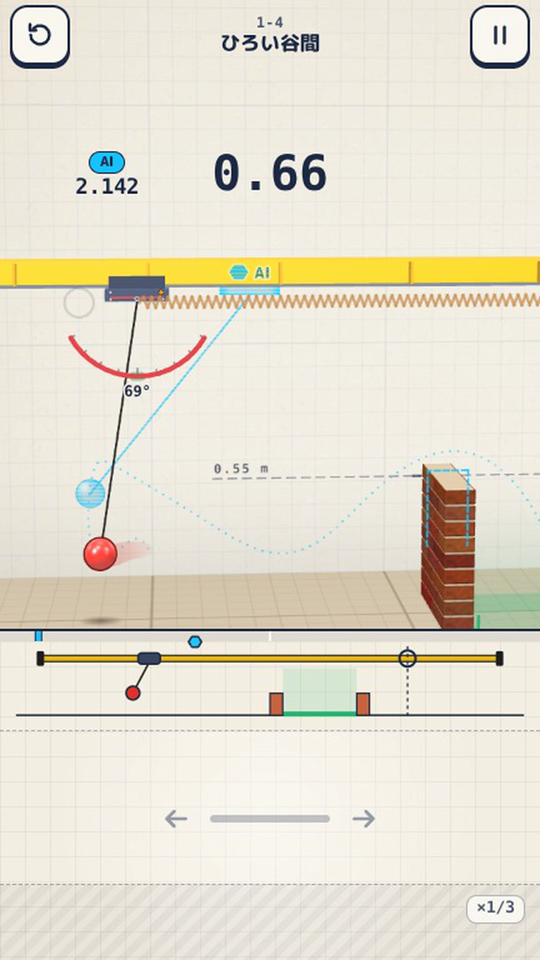
\includegraphics[width=\linewidth]{figs/shot_play.png}\caption{1-4 のプレイ}\end{subfigure}\hfill
\begin{subfigure}{0.24\linewidth}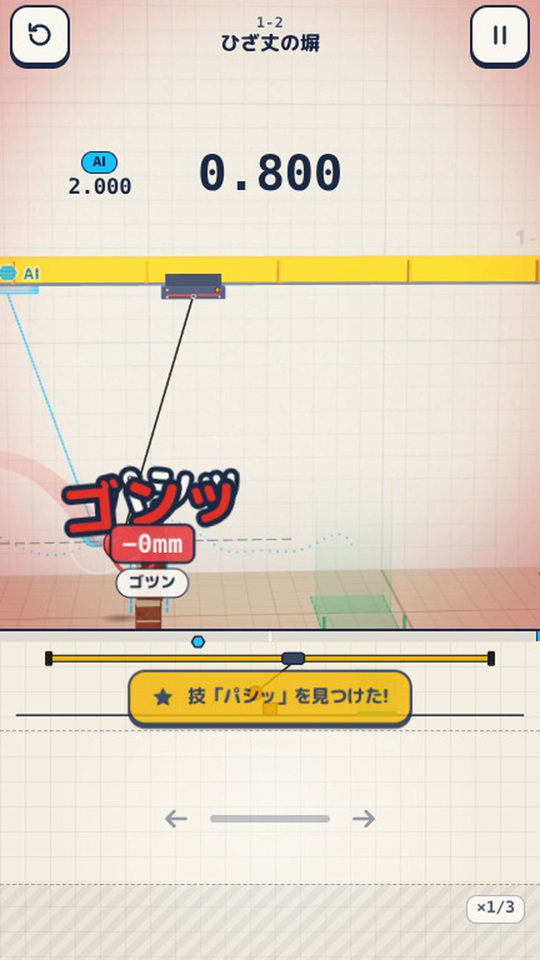
\includegraphics[width=\linewidth]{figs/shot_crash.png}\caption{1-2 で激突}\end{subfigure}\hfill
\begin{subfigure}{0.24\linewidth}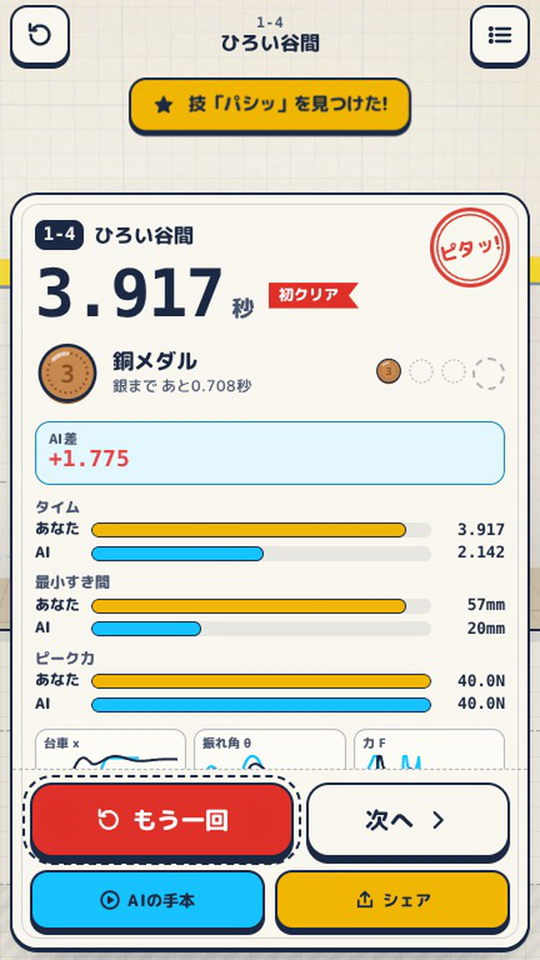
\includegraphics[width=\linewidth]{figs/shot_result.png}\caption{結果カード}\end{subfigure}\hfill
\begin{subfigure}{0.24\linewidth}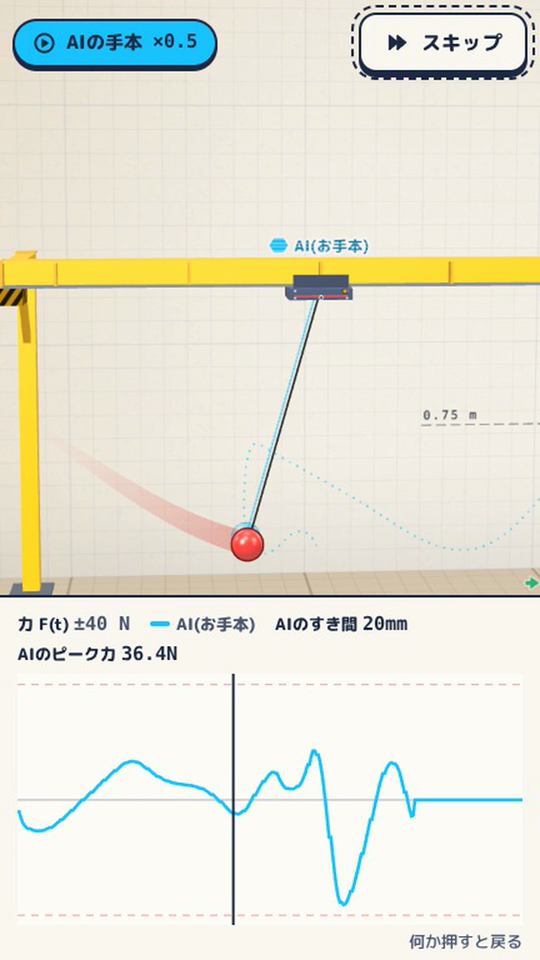
\includegraphics[width=\linewidth]{figs/shot_ai.png}\caption{2-2 の AI の手本}\end{subfigure}
\caption{完成したゲームの画面（宣伝動画用に実際の操作で録画した映像から切り出し）．
下半分が指で操作する盤，上の数字が AI と自分のタイム．(d) の下のグラフは AI が掛けた力 $F(t)$．}
\label{fig:shots}
\end{figure}

\section{成果物の規模と反響}
\label{sec:reception}

\subsection{規模}
\tabref{tab:size}に，公開時点のコードの規模を示す．
設計段階の前置きでは「全体で 5〜15k 行でよい」と書いていたが，テストを含めて約 5.5 万行になった．
そのうち約 1.9 万行がテストである．

\begin{table}[H]
\centering
\caption{公開時点のコードの行数（\code{game/} 以下）}
\label{tab:size}
\small
\begin{tabular}{lr@{\hspace{3em}}lr}
\toprule
部分 & 行数 & 部分 & 行数 \\
\midrule
UI（\code{src/ui}） & 10,323 & 音（\code{src/audio}） & 1,871 \\
ゲーム進行（\code{src/core}） & 4,563 & 入力（\code{src/input}） & 1,615 \\
描画（\code{src/render}） & 4,286 & Worker & 1,565 \\
Python ツール（\code{tools}） & 3,327 & 保存・通信・共有 & 1,810 \\
開発用デモ（\code{dev}） & 2,825 & テスト（\code{tests}） & 18,793 \\
物理（\code{src/sim}） & 2,430 & 設計書（\code{GAME\_DESIGN.md}） & 2,337 \\
\bottomrule
\end{tabular}
\end{table}

中身は次のとおりである．
\begin{itemize}
  \item 5ワールド 18 面．全面に，研究の最適化器で解いた AI のゴーストとパー（AI のタイム）がある．
  \item 最適化器で解いた日替わり用の 84 面と，Wordle 風の共有文つきの「今日の5球」．
  \item 物理は研究コードと同じ運動方程式に，紐のたるみ，張り直しの撃力，レール端の衝突を足したもの．
  sin/cos を自前で実装し，Chromium・Firefox・WebKit・Cloudflare workerd で結果がビット単位で一致する．
  \item Cloudflare Worker と D1 による面ごとの世界ランキング．送られた入力列をサーバーが同じ物理で再計算して検証する．
  \item 効果音はすべて WebAudio の合成，テクスチャはすべてプログラムで生成し，外部の素材ファイルはない．
\end{itemize}

\subsection{反響}
公開日（2026-09-23 JST）の全体が終わった直後（09-24 00:24 JST）に，Cloudflare の分析 API（GraphQL）から Worker と静的ファイル配信の要求数を，
本番の D1 から端末数を，いずれも読み取り専用で取得した（\tabref{tab:reception}）．
公開は 11:59 なので，公開日の数値は約 12 時間ぶんである．

\begin{table}[H]
\centering
\caption{公開日（9/23 JST，約 12 時間）の反響．上3行は Cloudflare の分析 API，下2行は本番 D1（9/24 00:24 時点）}
\label{tab:reception}
\small
\begin{tabular}{lr}
\toprule
項目 & 値 \\
\midrule
Worker の実行回数（\code{/api/*} の要求．エラー 0） & 23,505 \\
\quad 最も多かった 1 時間（16 時台） & 4,364 \\
静的ファイルの配信要求（HTML・JS・CSS．99.5\% がキャッシュから） & 24,673 \\
クリアの記録が届いた端末（重複なし） & 2,342 \\
面 1-1 / 1-2 / 1-3 / 1-4 / 2-1 をクリアした端末 & 1,729 / 1,264 / 1,044 / 633 / 557 \\
\bottomrule
\end{tabular}
\end{table}

数値の読み方は次のとおりである．
\begin{itemize}
  \item \texttt{workers.dev} のサブドメインで公開しているため，ゾーンの訪問者分析はなく，訪問者数そのものは取れない．
  最も近い値は，クリアの記録が届いた端末数である．
  \item 端末数は D1 の \code{plays} 表による．この表は公開当日の 20:44 に追加したもので，それ以前はランキング上位 100 位に入るか AI に初めて勝った走行しか残っていない．
  また，1つもクリアしなかった人や，オフラインで遊んだ人は数えない．したがって 2,342 は遊んだ端末数の下限である．1人が2台で遊べば2と数える．
  \item 開発中に D1 の自前カウンタで数えた値（20:31 時点で 11,754 件）は，Worker が要求数をまとめて書き込む方式のため少なめに出ていた．上の表では Cloudflare の分析 API の値を使った．
\end{itemize}

公開日の Worker 実行回数は Workers の無料枠（1日 10 万）の約 24\% で，
設計段階で見積もった「1日 2 万人が遊んでも無料枠に収まる」範囲に入っている．

\subsection{公開後の推移}
\label{sec:decay}
公開から約 2 日後の 2026-09-25 17:07 JST に，同じ方法（Cloudflare の分析 API と本番 D1．いずれも読み取り専用）で数値を取り直した．
1時間ごとの推移を\figref{fig:players}に，日ごとの値を\tabref{tab:daily}に示す．
データは \code{players\_timeseries.json}，図は \code{make\_players\_fig.py} で作った．

\begin{figure}[H]
\centering
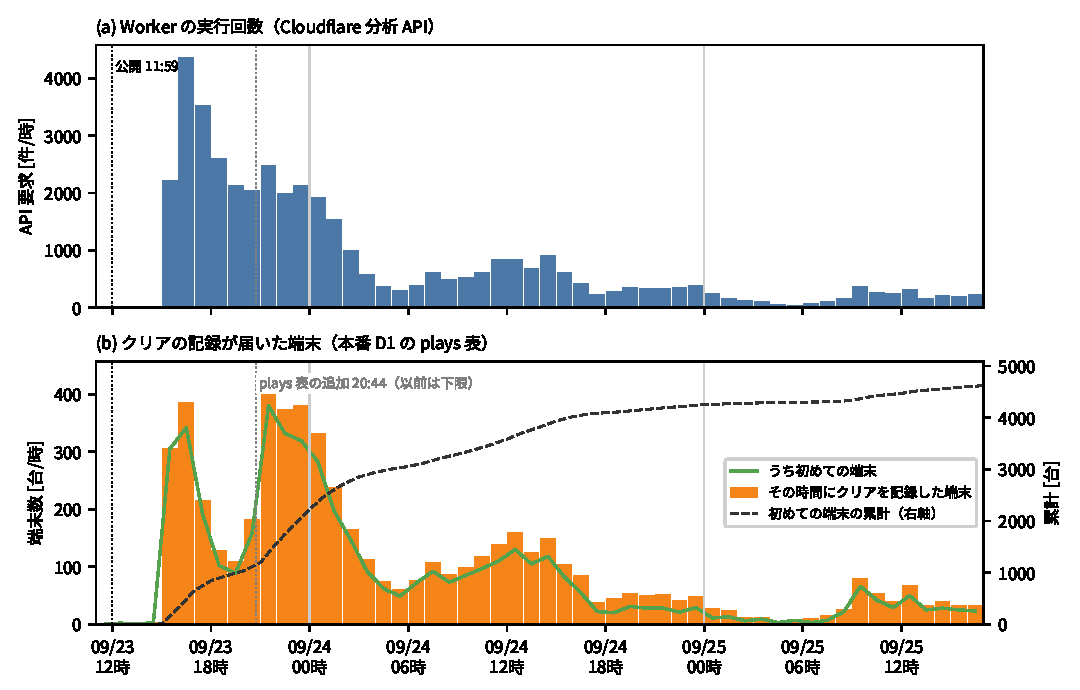
\includegraphics[width=\linewidth]{figs/players.pdf}
\caption{公開後のプレイヤー数の推移（1時間ごと，JST）．(a) Worker の実行回数．(b) その時間にクリアの記録が届いた端末数（棒），
そのうち初めて記録が届いた端末数（緑）と，その累計（破線，右軸）．9/25 は 17 時までの完全な時間だけを描いた．
plays 表は 9/23 20:44 に追加したので，それ以前の値は下限である．}
\label{fig:players}
\end{figure}

\begin{table}[H]
\centering
\caption{日ごとの推移（JST）．端末数は plays 表だけから数えたため，\tabref{tab:reception}の 2,342（runs 表との和）とは少し違う}
\label{tab:daily}
\small
\begin{tabular}{lrrr}
\toprule
日 & Worker 実行回数 & 静的ファイルの配信要求 & 初めて記録が届いた端末 \\
\midrule
9/23（公開日，11:59〜） & 23,505 & 24,673 & 2,223 \\
9/24 & 14,871 & 15,256 & 2,028 \\
9/25（17 時まで） & 3,045 & 3,931 & 369 \\
\midrule
累計（重複なし） & & & 4,624 \\
\bottomrule
\end{tabular}
\end{table}

\begin{itemize}
  \item \textbf{ピークは公開の約 4 時間後}（9/23 16 時台，4,366 件/時）で，その夜（21 時台）にも2つ目の山がある．
  9/24 の昼にも小さな山が出たが，9/25 の日中は 1時間あたり 150〜360 件で，ピークの 3〜8\% に落ちた．
  \item \textbf{新しく来る人は減り続けている}．初めて記録が届いた端末は 9/23 に 2,223 台，9/24 に 2,028 台だったが，
  9/25 は 17 時までで 369 台（1時間あたり 20〜60 台）である．累計の曲線は 9/25 の未明にほぼ平らになった．
  \item \textbf{戻ってくる人は少ない}．累計 4,624 台のうち，最初の記録と別の日（JST）にも記録が届いた端末は 244 台（5.3\%），
  最初の記録から 24 時間以上たって記録が届いた端末は 79 台（1.7\%）だった．
  plays 表は「面ごとの初回のクリア」しか残さないので，クリア済みの面だけを遊び直した人は数えられず，これは下限である．
  ただし「今日の5球」は日ごとに別の面として記録されるので，日替わりを遊びに戻った人はここに入る．
  Wordle 風の日替わりは再訪の仕掛けとして設計されたが（\secref{sec:ux}），少なくとも最初の2日間ではほとんど効いていない．
\end{itemize}

\section{考察}

\subsection{完成度を上げた工夫}
記録から読み取れる工夫を，役割ごとにまとめる．

\paragraph{判断を分ける}
\begin{itemize}
  \item 最初から1案に決めず，方向の違う5案を独立に作らせ，観点の違う3人に採点させた．重みは楽しさを最も重くした．
  \item 設計書を「互いに話さずに並行して作れるほど正確に」書かせ，次に「明日から作る主任エンジニア」の立場で批評させた．
  批評役は数値を自分で測り直し，解けない面や無料枠の超過を実装の前に見つけた．
  \item 指揮役はコードを書かず，各担当の報告を読んで決定事項（D1〜D10，R5〜R10）を出す役に徹した．
\end{itemize}

\paragraph{並行させても壊れない形にする}
\begin{itemize}
  \item 契約（型）と全ファイルの仮実装を先に作り，全体が型チェックを通る状態から並列実装を始めた．
  \item ファイルの所有者を1人に決め，他人のファイルが必要なら報告に「依頼」として書かせた．git の状態を変える操作と npm install を禁じた．
  \item テスト用サーバーのポート番号とビルドの出力先を担当ごとに分け，同時に動いても衝突しないようにした．
  \item 時間のかかる計算は，仮の結果を先に出して他を待たせず，本番の計算を裏で流した．
  \item 台本の中で依存関係を表し，レビューは物理コアの完成を待ってから始めた．
\end{itemize}

\paragraph{自己申告を信用しない}
\begin{itemize}
  \item 作る役と確かめる役を必ず分けた（土台の検証役，モジュールごとのレビュー役，総点検の反証役，CasADi の確認役）．
  \item 指摘には具体的な失敗の筋書きを求め，反証役には「裏付けられなければ偽とせよ」と指示した．
  \item 修正には回帰テストを付け，そのテストが元のコードで落ちることも確かめた．
  \item 「テストを弱めない」「根本原因を直す」を繰り返し指示した．
  \item 出力を JSON スキーマで固定し，受け入れ基準ごとに「通ったか」と「証拠」を書かせた．
\end{itemize}

\paragraph{目で見る，遊ばせる}
\begin{itemize}
  \item 描画・UI・統合の担当には，スクリーンショットを撮って画像として読み，直すことを繰り返させた．
  \item 人の代わりに，人間らしい制約とぶれをもつボットにゲームを遊ばせ，メダルの取りやすさを数値で測った．
  \item 面白さを「技」「最初の 60 秒の台本」「リトライ 100 ms 未満」のような検証できる仕組みに分解し，受け入れ基準に落とした．
  \item 見た目の基準（「AI っぽくしない」「スマホで読めるまで直す」）を言葉で与え，延べ 559 回のスクリーンショットの目視で詰めた．
\end{itemize}

\subsection{人が必要だったところ}
公開までの人の関与は\tabref{tab:human}の約 10 回で，大半は公開先や公開操作に関わるものだった．
その中で，ゲームの出来を最も大きく変えたのは試遊の感想（H7）である．
エージェントの審査は「『ピタッ』は腕の見せ所」を重く見て自動のゆれ止めを補助扱いに下げ，
ボットによる調査はキーボードの弱点を数値で示したものの，直すところまでは行かなかった．
実際に遊んだ人の「減衰させようとすると加速する」という一言が，それを覆した．
ボットは「画面を見ながら指で調整する感じ」までは再現できない，と指揮役自身も報告の中で述べていた．

また，外部に影響する操作（デプロイ，公開後に変えられない日付の決定）は，指揮役が必ず人に確認した．
CasADi の件では，人のヒントをそのまま採用せず，検証したうえで「いまは使わない」と判断し，理由（ライセンス）を示した．

\subsection{AI はなぜ面白さを扱えたのか}
\label{sec:whyfun}
公開後の数字（2日で 4,600 台以上，1-1 をクリアした端末の約 3 割が 2-1 までクリア）を見るかぎり，
少なくとも「一度遊んでみたくなり，数面は続けたくなる」面白さは作れていた．
しかし\secref{sec:fun}で見たとおり，エージェントは一度もゲームを「遊んで楽しんで」はいない．
それでも面白さを扱えた理由は，記録から次の4つにまとめられる．

\paragraph{1. 面白さを既知の型の組み合わせとして扱った}
5案の方向づけのプロンプトは，すべて既存の作品を参照点にしている
（Trackmania，Getting Over It，QWOP，Tiny Wings，Downwell，Vlambeer の ``juice it or lose it''，Portal，Baba Is You，Wordle）．
審査役の講評も「Trackmania 型の即リトライ」「Wordle 風の共有行」のように，型の名前で面白さを語っている．
言語モデルは，こうした作品についての大量の批評や設計論を学んでおり，
「どの仕組みがどんな感情を生むか」を言葉の上では知っている．
エージェントがしたのは，面白さを体験することではなく，既知の型を題材に合わせて選び，組み合わせることだった．

\paragraph{2. 題材が面白さの核をすでに持っていた}
研究コードには，本物の最短時間の最適化器があった．
3人の審査役がそろって mastery 案を選び，忠実さの軸で 29/30 を付けたのは，「本物の最適制御 AI と競う」がほかでは作れない核だったからである．
AI の 2 cm の余裕は「人間は 0 mm まで攻めてよい」という勝ち筋に，紐のたるみは「パシッ」という技になった．
エージェントは面白さを無から作ったのではなく，題材に埋まっていた面白さを見つけて，ゲームの規則に翻訳した．
翻訳の筋は「AI は規則を守る．人は規則の隙間を使ってよい」という1文にまとまっており，これが3本の柱すべてを貫いている．

\paragraph{3. 面白さを検証できる仕組みに分解した}
「最初の 60 秒」は秒単位の台本に，「もう一回」は「リトライ 100 ms 未満」に，「緊張」は「すき間を mm で表示し，20 mm の論文ラインを引く」に落とされた（\secref{sec:fun-gdd}）．
こうすると，面白さそのものは測れなくても，面白さを支えるはずの仕組みが「あるか，動くか」はテストで確かめられる．
エージェントの強みである「大量に確かめる」を，面白さにも使える形にしたことになる．

\paragraph{4. 1人の好みではなく，観点の違う合議にした}
案を5つ出して観点の違う3人に採点させたことで，1体の思いつきに依存しなかった．
楽しさの軸では arcade が1位だったが，作りやすさと合わせた合計で mastery が選ばれ，arcade の良い部分（すき間の mm 表示，相対ドラッグ）は移植された．

\paragraph{限界：手触りと「また来たい」は扱えなかった}
一方で，操作の手触り（キーを押すと加速しすぎる）は人の試遊まで見つからなかった（\secref{sec:human}）．
審査役「プレイヤー」には ``whether you would come back tomorrow''（明日もまた来たいか）を評価させていたが，
実際に別の日に戻ってきた端末は約 5\% だった（\secref{sec:decay}）．
文章の上で評価できる面白さ（初見の引き，共有したくなる物語）は当たり，
遊んで初めてわかる面白さ（手触り）や，時間をかけて初めてわかる面白さ（習慣になるか）は外れた．
「AI は面白さを理解した」というより，「AI は面白さを，言葉で説明できる範囲で再構成できた」と言うのが正確だと考える．

\subsection{丸投げか，仕様の言語化の移譲か}
\label{sec:delegate}
公開後，X で「丸投げに見えて，実は仕様の言語化を AI に移譲している」「人が先に決めようとする制約が抜け落ちるぶん，構造がすっきりする」
「何を作るかより，どう問いを渡すかが本質」という趣旨の感想をもらった．記録に照らして検討する．

\paragraph{言語化の移譲：記録はおおむねこれを支持する}
人が書いたのは2文（約 50 文字）である．これに対し，指揮役とサブエージェントが書いた仕様は，
ワークフローの台本6本で約 9.6 万文字（英語），設計書 \code{GAME\_DESIGN.md} で 2,337 行，これに決定事項 D1〜D10，R5〜R10 が加わる．
ジャンル，対象の端末，操作方式，面の寸法，失敗の規則，ランキングの仕組み，色の値，効果音のレシピまで，すべてエージェントが言葉にした．
「何を作るか」の言語化は，ほぼすべて移譲されたと言ってよい．

\paragraph{制約が抜け落ちると構造がすっきりするか：半分正しい}
人がジャンルも規模も決めなかったので，指揮役は設計の空間を5方向に開いたまま探索できた．
入った制約は，人の好みではなく目的と題材から導かれたもの（研究と同じ運動方程式，無料枠，再シミュレーションのためのビット単位の決定性）で，
それぞれに理由があるので，設計書の構造は一貫している．この点で感想は当たっている．

ただし，制約が「なかった」わけではない．指揮役は前置き（\lstref{lst:context}）に，規模（5〜15k 行），「技術デモではなく本当に面白いもの」，
オフラインで動くこと，など多くの制約を\textbf{自分で書き足して}いる．抜け落ちたのは「人が先に決める制約」で，制約そのものは AI が書いた．
また，AI が導けない種類の制約もあった．
\begin{itemize}
  \item \textbf{外の世界の制約}：公開先（H2）は9分遅れで届き，最初の設計ワークフローを止めてやり直した（5体，約 39 万トークン）．
  公開先，予算，権利（CasADi の METIS のライセンスは AI が自分で見つけたが）など，外から与えられる条件は，先に言うほど安い．
  \item \textbf{体験から出る制約}：「難しすぎる」（H7）は，遊んだ人にしか言えない．
\end{itemize}
つまり，移譲してよいのは「目的から導ける制約の言語化」で，「外の世界の条件」と「体験による判定」は人が持ち続ける必要があった．

\paragraph{「どう問いを渡すか」：指揮役自身がそれをしていた}
この感想は，人と指揮役の間だけでなく，指揮役とサブエージェントの間にも当てはまる．
指揮役の仕事の大部分は，コードを書くことではなく，問いの形を決めることだった．
\begin{itemize}
  \item 「人間は最適制御 AI に勝てるか？」（mastery 案への問い）
  \item 「メダルの基準は\textbf{人間}に達成できるか？」（難易度調査役への問い）
  \item 「この指摘を\textbf{反証}せよ．裏付けられなければ偽とせよ」（反証役への問い）
  \item 「明日から作り始める主任エンジニアとして，抜けを探せ」（批評役への問い）
\end{itemize}
問いの形が，出てくるものの質を決めていた．
その裏返しとして，\textbf{問われなかったことは作られなかった}．
最初の依頼は「最強に面白い」で，「長く遊ばれる」「続けて運営できる」は問われていない．
エージェントたちも再訪を主な評価軸にしなかった．結果として，一度遊ぶ面白さは作れたが，持続性はほぼゼロだった（\secref{sec:sustain}）．
「どう問うか」が本質だという主張は，良い面と悪い面の両方で，今回の記録によく当てはまる．

さらに付け加えると，今回の問いは2文だけではなかった．問いと一緒に，研究コード（運動方程式，最適化器，検証済みの数値）という大きな「答えの材料」を渡している．
2文の依頼だけを空のリポジトリで出していたら，面白さの核（本物の AI と競う）は生まれなかった可能性が高い．
「丸投げ」が成り立ったのは，問いが短かったからではなく，問いの背後にある材料が厚かったからでもある．

\subsection{役割分担，レビューの境界，失敗時の止め方}
\label{sec:roles}
別の読者から，役割分担，レビューの境界，失敗したときの停止条件を確かめたい，という声があった．
台本から読み取れるものを\tabref{tab:roles}にまとめる．

\begin{table}[H]
\centering
\caption{役割ごとの書き込み範囲と，その出力を確かめる役（台本から整理）}
\label{tab:roles}
\small
\begin{tabularx}{\linewidth}{>{\raggedright\arraybackslash}p{0.2\linewidth}>{\raggedright\arraybackslash}X>{\raggedright\arraybackslash}p{0.27\linewidth}}
\toprule
役割 & 書いてよい範囲 & 出力を確かめる役 \\
\midrule
指揮役 & 台本と決定事項だけ（コードは書かない） & 人（外部に影響する操作は必ず確認） \\
案を作る役（①） & 何も書かない（JSON を返すだけ） & 審査役3人 \\
審査役（①） & 何も書かない & 指揮役（重み付き合計） \\
統合役・批評役（①） & 設計書1ファイル & 批評役 → 指揮役 \\
土台の担当（②） & 雛形と仮実装，面データ & 検証役（全コマンドを自分で再実行） \\
モジュール担当 O1〜O9（③） & 所有ファイルだけ．他人のファイルは「依頼」として報告 & 同じファイルを引き継ぐレビュー兼修正役 \\
修正役（④） & 所有ファイルだけ & 統合役（全ファイルを引き継ぎ，全テスト） \\
難易度調査役（④⑤） & 作業用の一時ディレクトリだけ（ゲームは読み取り専用） & 指揮役（R5〜R10 を決める） \\
粗探し役（⑤） & 何も書かない（読み取り専用） & 反証役（1件ごとに別の1体） \\
反証役（⑤） & 一時ディレクトリだけ & 修正役（確定した指摘だけを受け取る） \\
修正役（⑤） & 観点ごとに重ならないファイル & ゲート役（全テストと難易度の再測定） \\
\bottomrule
\end{tabularx}
\end{table}

\paragraph{レビューの境界} 境界の引き方には，3つの原則が見える．
第一に，\textbf{作る役と確かめる役は必ず別の個体}である．同じモデルでも，文脈を共有しない別の個体に確かめさせた．
第二に，\textbf{書き込み範囲をファイル単位で分けた}．並行する役どうしの書き込み範囲は重ならず，レビュー役は元の担当と「同じファイルだけ」を引き継ぐ．
確かめるだけの役（粗探し，反証，難易度調査）は，ゲームのソースに書き込めない．
第三に，\textbf{境界を越える変更は報告で上に上げる}．他人のファイルの変更が必要なときは \code{requests\_for\_other\_owners} に書き，
指揮役がそれを裁定して次の台本の決定事項にした．
全員に共通の禁止事項として，git の状態を変える操作，\code{npm install}，\code{game/} の外への書き込みがあった．

\paragraph{失敗時の止め方：自動の停止条件はほとんどなかった}
この点は正直に書く必要がある．台本には，「この条件なら全体を止める」という停止条件は\textbf{ほぼ書かれていない}．
台本は失敗を吸収して先へ進む作りになっている．
\begin{itemize}
  \item エージェントが失敗すると結果は \code{null} になり，\code{filter(Boolean)} で落として次の段へ進む（例：5案のうち1つが失敗しても，残りで審査する）．
  \item モジュールの作成が失敗しても例外を捕まえて \code{\{key, error\}} を返し，ほかのモジュールは続ける．
\end{itemize}
代わりに，次のものが止める役を果たしていた．
\begin{itemize}
  \item \textbf{ワークフローの切れ目}：7本のワークフローは1本ずつ指揮役に結果を返す．指揮役は報告を読み，スクリーンショットを見て，次の台本を書く．
  実質的な停止条件の判断はここで行われた．最初の設計ワークフローを止めたのもこの判断である（H2 を受けて中止）．
  \item \textbf{ゲート}：各工程の最後の役（統合役，ゲート役）は「全テストが通るまで直す．根本原因を直し，テストを弱めない」ことを求められた．
  これは停止条件ではなく完了条件だが，通らなければ報告の \code{open\_problems} に残る．
  \item \textbf{時間と計算の上限}：難易度調査は「全体で約 60 分」，最適化器は候補ごとにプロセスを打ち切り，時間切れの候補は1回だけ延長して解き直す．
  \item \textbf{正直な報告の要求}：全員に ``Report failures honestly''（失敗は正直に報告せよ）と，受け入れ基準ごとの「通ったか」と「証拠」を書かせた．
  失敗を隠さずに上げさせることが，止める判断の前提になっている．
  \item \textbf{外部に影響する操作は人の承認}：デプロイ，公開後に変えられない日付，リポジトリの接続は人が行った．
\end{itemize}
この設計は，今回のように「壊れても作業ツリーの中で閉じる」開発では機能した．
しかし，エージェントが失敗しても黙って先へ進むので，たとえば9体のモジュール担当のうち物理コア（全員が依存する）が失敗した場合でも，
台本はレビューを始めてしまう（\lstref{lst:pipeline} は物理コアの失敗を \code{null} として待つだけで，止まらない）．
今回それが起きなかったのは結果論である．
次に同じことをするなら，「依存の根っこが失敗したら下流を止める」「ゲートが通らなければ次のワークフローに進まない」を台本に明示すべきだと考える．

\subsection{持続可能性と将来性}
\label{sec:sustain}
\figref{fig:players}は，X の投稿の拡散とともに人が来て，拡散が収まるとともに去っていく形をしている．
筆者は，このまま拡散が終われば，プレイ人口はほぼゼロになると考えている．
本節では，「持続可能なゲーム」をこのゲームの外側の問題として考える．

\paragraph{2つの持続可能性} 持続可能性には2つの意味がある．
\begin{itemize}
  \item \textbf{運営の持続}：このゲームはほぼ満たしている．サーバーは Cloudflare の無料枠の中で動き，
  拡散のピークの日でも Worker の実行回数は上限の約 24\% だった．保守の必要な常駐のサーバーもない．
  誰も遊ばなくなっても費用はかからないので，「作品」としては何年でも置いておける．
  \item \textbf{プレイ人口の持続}：こちらはほぼゼロである．再訪率は 1〜5\% で，新規は拡散の波が来たときだけ入ってくる．
  ゲームとして生き続けるには，拡散がなくても毎日遊びに来る人が一定数いる状態が要るが，その兆しは見えない．
\end{itemize}
「持続可能なゲームを作る」は，「面白いゲームを作る」とは難しさの段階がいくつも違う，というのが筆者の実感である．
今回，AI エージェントは後者の壁を大きく下げた．約 14 時間，人の指示約 10 回で，拡散されて 2 日で 4,600 台以上に遊ばれるものができた．
しかし前者，つまり人が習慣として戻ってくる理由や，運営を続けるための収入は，開発の自動化では下がっていない．
作る費用が下がるほど，差がつくのは「作ったあと」になる．

\paragraph{収益化：広告は付けられない} 収益の手段として最初に思いつくのは広告だが，このゲームには合わないと考える．
\begin{itemize}
  \item このゲームの売りは「リトライは 100 ms 未満で，読み込みもカウントダウンもない」「30 秒しか我慢しない人に最初の 10 秒で伝わる」ことである（\secref{sec:fun}）．
  リトライの間や結果画面に広告を挟めば，売りそのものを壊す．
  \item 縦画面の下 38\% は指で操作する盤で，上は 3D の場面と HUD で埋まっている．バナーを置く場所は，操作か視認性のどちらかを削らないと作れない．
  \item 遊ぶ時間は1人あたり数分で，再訪もほとんどない．表示回数が拡散の日に集中し，その後は残らないので，広告の収入も同じ形で一瞬で終わる．
\end{itemize}
つまり，広告を付けると遊ばれなくなり，付けなければ収入がない．今の形のままでは，収益による持続はほぼ見込めない．

\paragraph{ウェブアプリであること} ウェブアプリであることは，拡散では強みで，定着では弱みだった．
\begin{itemize}
  \item \textbf{強み}：X のリンクを押せば 1〜2 秒で遊べる．インストールもアカウントも要らない．
  「30 秒しか我慢しない」人を取りこぼさないこの摩擦の低さが，公開2日で 4,600 台以上という数字を生んだと考えられる．
  \item \textbf{弱み}：遊び終えたタブを閉じると，戻ってくるきっかけが何も残らない．
  ホーム画面のアイコンも，「今日の5球が更新された」という通知もない．保存は端末のブラウザの中だけにある．
\end{itemize}

\paragraph{スマホのネイティブアプリにしていたら} ネイティブアプリにすれば，定着の弱みの一部は改善したと考える．
ホーム画面のアイコンは毎日目に入り，プッシュ通知で日替わりを知らせられ，ストアの検索や「おすすめ」という，拡散以外の新規の入り口もできる．
課金（広告を消す買い切り，スキン）もストアの仕組みで扱いやすい．
一方で，インストールという一手間が入ると，拡散の瞬間に来た人の大半は遊ぶ前に離れた可能性が高い．
ストアの審査，年間の登録料，手数料（15〜30\%）もかかる．
したがって「最初からネイティブ」より，「ウェブで拡散させ，気に入った人をアプリに移す」二段構えが現実的だったと考える．
その中間として，PWA（ホーム画面への追加と Web Push．iOS も 16.4 以降は対応）はコードをほぼ変えずに試せる．
描画は three.js，物理と不正対策は TypeScript なので，Capacitor などでアプリに包むことも技術的には難しくない．

\paragraph{将来性} プレイ人口を持続させる方向として，次が考えられる．
\begin{itemize}
  \item \textbf{コンテンツを出し続ける}：面の追加を定期的に行う．①で「作りやすさ」を理由に削った面エディタ（sandbox 案）と，URL で共有できる面は，
  作り手を遊び手の側に増やす，最も長く効く仕掛けである．AI エージェントで作る費用が下がった今，削った機能を後から足す判断は以前より軽い．
  \item \textbf{イベントで波を作り直す}：「人類 vs AI」の集計（AI に勝った人数），期間限定の面，世界記録の更新の告知など，
  拡散のきっかけを周期的に作る．1回の大きな波ではなく，小さな波を何度も起こす運営である．
  \item \textbf{教材として置く}：このゲームは研究の最適制御と同じ運動方程式の上にある．
  劣駆動系，共振，最短時間制御を「指で体験してから式を見る」教材は，大学や高専の授業という，拡散に頼らない利用者を持ちうる．
  娯楽としての持続よりも，こちらのほうが今回の出自に合っている．
  \item \textbf{作品として割り切る}：運営費がほぼゼロなので，プレイ人口の持続を目標にせず，
  「研究を 2 日で数千人に触ってもらった」ことを成果とする考え方もある．本稿は，実質的にこの立場で評価している．
\end{itemize}

\subsection{費用と限界}
\label{sec:limits}
\begin{itemize}
  \item 規模：開発セッションだけで 70 体，ツール呼び出し 5,921 回，約 1,900 万トークンを使った．
  個人の趣味の開発としては大きく，ultracode を選んだ時点でこの規模を許したことになる．
  \item 時間：開発セッションは約 14.4 時間で，そのうちの多くはエージェントが裏で動いている時間だった．
  最適化器の計算（本番ゴースト 84 分，日替わりの解き直し 2 時間 44 分）が工程の長さを決めていた．
  \item 規模の見積もり：前置きでは 5〜15k 行としていたが，テストを含めて約 5.5 万行になった．
  \item 本稿の偏り：本稿の分析と執筆は Claude Code が行った．数値はすべて記録から集計したものだが，
  「工夫」の選び方や評価には，作った側の視点が入りうる．
  \item 面白さの評価：点数が付いたのは文書（案の JSON）に対する審査だけで，遊んだうえでの評価ではない．
  楽しさの軸は5案で差がつきにくく，順位は作りやすさで決まった．手触りの問題は人の試遊まで見つからなかった．
  \item 持続性の評価：公開から約2日しかたっておらず，再訪率は最初の2日だけの値である．また plays 表は面ごとの初回のクリアしか残さないので，再訪は過小に数えている．
  \item 反響の数値：訪問者数は取れず，端末数はクリアの記録が届いたものに限られるので，\tabref{tab:reception}の端末数は遊んだ人数の下限にすぎない．
\end{itemize}

\section{まとめ}
2文の依頼から，Claude Code は 7 本のワークフローで 70 体のサブエージェントを動かし，
約 14 時間で，研究の最適化器を競走相手にしたブラウザゲームを設計・実装・検証した．
進め方の要点は，複数案と審査による設計，契約と仮実装の先行，所有権を分けた並列実装，
作る役と確かめる役の分離，そしてスクリーンショットとボットによる「見て，遊ばせて」確かめることだった．
人の関与は約 10 回で，ゲームの出来を最も大きく変えたのは，実際に遊んだ人の「難しすぎる」という一言だった．
公開日の約 12 時間で，API 要求は 23,505 件，クリアの記録が届いた端末は少なくとも 2,342 台だった．
ただし2日後にはピークの数\%まで落ち，別の日に戻ってきた端末は約 5\% にとどまった．
AI エージェントは「面白いものを作る」費用を大きく下げたが，「遊ばれ続ける」ための仕組みと収益は，広告が売りの速さと両立しないこともあり，今回は解けていない．
ウェブで拡散させ，PWA やネイティブアプリ，教材としての利用で定着させることが，次の課題である．
また，今回の「丸投げ」は，実際には仕様の言語化を AI に移譲し，人は外の世界の条件と体験による判定を持ち続ける分担だった．
何が作られるかは問いの形で決まり，問われなかった「持続」は作られなかった．
台本には自動の停止条件がほとんどなく，止める判断はワークフローの切れ目で指揮役が担っていた．

\begin{thebibliography}{9}
\bibitem{gulley2026} N.~Gulley, ``Simulate in MATLAB, Animate in Blender,'' MathWorks Blogs, 2026.
\bibitem{kaibuchi2026} 貝淵蒼馬，「吊り下げボールを壁の隙間に出し入れするガントリークレーン：軌道最適化・時変LQR・独立検証による再現」，
\url{https://github.com/Raptor-zip/crane-ball-wall}，2026．
\end{thebibliography}

\appendix
\section{面の一覧と AI のタイム}

\begin{table}[H]
\centering
\caption{18 面と AI のタイム（最適化器で求めた最短時間．ゲーム内の判定で測った値）}
\small
\begin{tabular}{llr@{\hspace{2em}}llr}
\toprule
面 & 名前 & AI [s] & 面 & 名前 & AI [s] \\
\midrule
1-1 & おつかい & 1.500 & 3-2 & 原典・ブランコ & 3.858 \\
1-2 & ひざ丈の塀 & 2.000 & 3-3 & 短い紐 & 4.125 \\
1-3 & 腰の高さ & 2.750 & 4-1 & ハードル走 & 4.375 \\
1-4 & ひろい谷間 & 2.142 & 4-2 & 終点 & 2.475 \\
2-1 & ブログの壁 & 2.742 & 4-3 & たまご & 3.100 \\
2-2 & 原典：いれる & 2.625 & 5-1 & 重い荷 & 2.192 \\
2-3 & 原典：だす & 2.650 & 5-2 & 階段ポケット & 2.633 \\
2-4 & 郵便受け & 2.075 & 5-3 & 天井すれすれ & 3.100 \\
3-1 & 非力モーター & 5.575 & 5-4 & フルコース & 5.775 \\
\bottomrule
\end{tabular}
\end{table}

\section{プロンプトの抜粋}

\begin{lstlisting}[caption={5案の方向づけ（mastery と mobile）}]
{ key: 'mastery', label: 'Mastery / beat-the-AI speedrun', brief: 'Design from the angle of a precision skill toy
  with deep mastery: tight, readable controls, fast retry, speedrun timers, ghost races against your best run AND
  against the trajectory optimiser ("AI"), medals. Think Trackmania / Getting Over It (but not cruel) / QWOP-lite
  physics mastery. The headline hook is "can a human beat the optimal-control AI?"' },
{ key: 'mobile', label: 'Mobile-first casual + social', brief: 'Design from the angle of a phone-first, one-thumb
  game with 30-second sessions and strong social hooks: instantly understandable touch control, daily challenge
  with a shared global leaderboard (Cloudflare Worker + D1), shareable result text for X (Wordle-style), async
  ghost races against other players. The first 10 seconds must be self-explanatory without text.' },
\end{lstlisting}
\begin{yaku}
mastery（熟達／AI に勝つスピードラン）：深い熟達のある精密な技能玩具という方向から設計せよ．
きびきびして読みやすい操作，速いリトライ，スピードランのタイマー，自己ベストと軌道最適化器（「AI」）の\textbf{両方}とのゴーストレース，メダル．
Trackmania，Getting Over It（ただし残酷にしない），QWOP を軽くしたような物理の熟達を思い浮かべよ．
一番の売りは「人間は最適制御 AI に勝てるか？」である．\\[3pt]
mobile（スマホ優先のカジュアル＋ソーシャル）：スマホ優先，親指1本，1回 30 秒，強いソーシャルの仕掛け，という方向から設計せよ．
すぐにわかるタッチ操作，共有の世界ランキングつきの日替わりチャレンジ（Cloudflare Worker + D1），X 向けの共有できる結果文（Wordle 風），ほかのプレイヤーとの非同期のゴーストレース．
最初の 10 秒は文章なしでわかるものにすること．
\end{yaku}

\begin{lstlisting}[caption={審査役「プレイヤー」の観点}]
You are the target player: a Japanese engineer/student who sees this on X, taps the link on a phone, and has 30
seconds of patience. Also imagine sharing it with friends. Judge on first-minute clarity, touch controls,
shareability, the "wow, this is the real physics from the paper" factor, and whether you would come back tomorrow.
\end{lstlisting}
\begin{yaku}
あなたは想定プレイヤーである．X でこれを見かけ，スマホでリンクをタップし，30 秒しか我慢しない日本の技術者・学生．友達に共有する場面も想像せよ．
最初の1分のわかりやすさ，タッチ操作，共有したくなるか，「すごい，論文の本物の物理だ」と思えるか，明日もまた来たいか，で評価せよ．
\end{yaku}

\begin{lstlisting}[caption={レビュー役への指示}]
# Your role: independent REVIEWER-FIXER for module ${m.key}
The owner agent just finished building this module. Its report: ${JSON.stringify(build)}
...
1. Adversarially review the module against GAME_DESIGN.md ... and against the quality bar (fun, feel, polish,
   robustness, performance, accessibility). Read ALL of the module's code. Look for: spec deviations, missing
   features, bugs, edge cases (NaN, empty data, null minGapMm, offline, rotated phone, reduced motion),
   non-determinism, allocation in hot loops, memory leaks, flaky tests, tests that do not really test the claim.
2. Run every test/check the module's acceptance criteria name (and add missing tests). For visual modules take
   screenshots and LOOK at them critically as a player on a phone would.
3. FIX everything you find directly in the module's files, re-run, and iterate until the acceptance criteria
   truly pass.
\end{lstlisting}
\begin{yaku}
\# あなたの役割：モジュール \$\{m.key\} の独立したレビュー兼修正役\\
担当エージェントがこのモジュールを作り終えたところである．その報告：\$\{JSON.stringify(build)\}\\
…\\
1. GAME\_DESIGN.md（…）と品質の基準（楽しさ，手触り，磨き込み，堅牢さ，性能，アクセシビリティ）に照らして，このモジュールを\textbf{敵対的に}レビューせよ．
モジュールのコードを\textbf{すべて}読むこと．探すもの：仕様からの逸脱，欠けている機能，バグ，端のケース（NaN，空のデータ，minGapMm が null，オフライン，スマホの回転，reduced motion），
非決定性，毎フレームの処理の中での確保，メモリリーク，不安定なテスト，主張を本当には確かめていないテスト．\\
2. モジュールの受け入れ基準が挙げるテスト・検査をすべて実行せよ（足りないテストは足すこと）．見た目のモジュールではスクリーンショットを撮り，スマホのプレイヤーの目で厳しく\textbf{見る}こと．\\
3. 見つけたものはすべて，モジュールのファイルで直接\textbf{直し}，実行し直し，受け入れ基準が本当に通るまで繰り返せ．
\end{yaku}

\begin{lstlisting}[caption={難易度調査役への指示（抜粋）}]
Question: are the medal thresholds (bronze <= 2.0*P, silver <= 1.5*P, gold <= 1.2*P, crown < P, with P = AI
parSub) achievable by HUMANS on each of the 18 campaign levels and on a sample of 12 daily levels?
Method: ... imports the real simulator (src/sim) and the real servo (src/input/servo.ts) and plays each level
with HUMAN-LIKE controller families:
 (a) touch/mouse: a target position x_t(t) that is piecewise linear with <= 6 knots, knot spacing >= 0.15 s,
     target speed <= 5 m/s, then held;
 (b) keyboard: velocity intents from {-4, 0, +4} m/s (and fine +-1) with the spec ramps, <= 7 switches ...
 plus a human reaction/precision penalty: add Gaussian timing jitter sigma = 40 ms and position jitter
 sigma = 1 cm to the best found plan and report the success rate over 50 jittered replays.
\end{lstlisting}
\begin{yaku}
問い：メダルの基準（銅 $\le 2.0P$，銀 $\le 1.5P$，金 $\le 1.2P$，王冠 $< P$．P は AI の parSub）は，キャンペーンの 18 面それぞれと日替わり面から選んだ 12 面で，\textbf{人間}が達成できるか？\\
方法：…本物のシミュレーター（src/sim）と本物のサーボ（src/input/servo.ts）を読み込み，人間らしい操作の族で各面を遊ぶ．\\
(a) タッチ／マウス：目標位置 $x_t(t)$ を折れ線とし，折れ点は 6 個以下，折れ点の間隔は 0.15 s 以上，目標の速さは 5 m/s 以下，その後は保持．\\
(b) キーボード：速度の意図を $\{-4, 0, +4\}$ m/s（と微速 $\pm 1$）から選び，仕様どおりの加減速，切り替えは 7 回以下…\\
さらに人間の反応と精度のペナルティとして，見つけた最良の操作に時刻のぶれ $\sigma = 40$ ms と位置のぶれ $\sigma = 1$ cm のガウス雑音を加え，50 回のぶれた再生での成功率を報告せよ．
\end{yaku}

\begin{lstlisting}[caption={審査役の出力スキーマ（採点部分）},label={lst:judgeschema}]
scores: { type: 'array', items: { type: 'object', properties: {
  angle: { type: 'string' },
  fun: { type: 'number', description: '0-10 moment-to-moment fun and replayability' },
  first_minute: { type: 'number', description: '0-10 how quickly a newcomer gets it and gets hooked' },
  feasibility: { type: 'number', description: '0-10 likelihood of a polished, bug-free result in one session' },
  originality: { type: 'number', description: '0-10' },
  fidelity: { type: 'number', description: '0-10 faithfulness to the research physics/story' },
  comment: { type: 'string' } } } },
recommended_base: { type: 'string', description: 'angle key of the best base concept' },
best_ideas_to_graft: [ { from, idea, why } ],  ideas_to_cut: [ { idea, why } ],
control_scheme_verdict: { type: 'string', description: 'which control scheme(s) to ship for desktop and touch and why' },
failure_rule_verdict: { type: 'string', description: 'what should happen on wall contact / slack string, and why' },
\end{lstlisting}
\begin{yaku}
scores（案ごとの点数）：angle（案のキー），
fun「0〜10．その瞬間瞬間の楽しさと，繰り返し遊びたくなるか」，
first\_minute「0〜10．初めての人がどれだけ早く理解し，はまるか」，
feasibility「0〜10．1セッションで磨き込まれ，バグのない結果になる見込み」，
originality「0〜10」，
fidelity「0〜10．研究の物理や物語への忠実さ」，comment（講評）．\\
recommended\_base「土台として最良の案のキー」，best\_ideas\_to\_graft（移植すべき案：出どころ，案，理由），ideas\_to\_cut（捨てる案：案，理由）．\\
control\_scheme\_verdict「デスクトップとタッチでどの操作方式を出荷するか，その理由」，
failure\_rule\_verdict「壁に触れたとき／紐がたるんだときにどうなるべきか，その理由」．
\end{yaku}

\begin{lstlisting}[caption={案を作る役への共通の指示と，案の出力スキーマの面白さに関わる項目}]
You are a senior game designer. ${a.brief}
Produce ONE complete game concept for this project (a single game, not a menu of options). Be concrete: real
numbers for level geometry in metres ... exact control mappings, exact success/failure rules. Give 12-20 levels.
... Aim for what a player would call 最強に面白い.
  pitch: '1 paragraph: what the player does and why it is fun'
  first_60_seconds: 'moment-by-moment what a first-time player experiences'
  juice_visual_audio, art_direction, why_most_fun, risks_and_mitigations
\end{lstlisting}
\begin{yaku}
あなたはシニアのゲームデザイナーである．\$\{a.brief\}\\
このプロジェクトのゲーム案を\textbf{1つ}，完全な形で作れ（選択肢の一覧ではなく，1本のゲーム）．具体的に書くこと：面の形はメートル単位の実数で…，操作の対応は正確に，成功と失敗の規則も正確に．面は 12〜20 個．
… プレイヤーが「最強に面白い」と呼ぶものを目指せ．\\
pitch「1段落：プレイヤーが何をするか，なぜそれが楽しいか」，
first\_60\_seconds「初めてのプレイヤーが体験することを瞬間ごとに」，
juice\_visual\_audio（演出の見た目と音），art\_direction（アートの方針），why\_most\_fun（なぜ最も面白いか），risks\_and\_mitigations（リスクと対策）．
\end{yaku}

\begin{lstlisting}[caption={審査役「作りやすさ」の観点（全文）}]
You are a principal engineer who will own the build (three.js, TypeScript, WebAudio, mobile web performance,
Cloudflare Workers + D1 backend within the free tier, anti-cheat re-simulation, single-file preview packaging,
physics integration, testing). Judge primarily on feasibility, risk of bugs, physics correctness (same EOM as the
Python code so optimiser ghosts are valid; slack string and collisions must be robust), and whether the scope
yields a POLISHED result rather than a broad buggy one.
\end{lstlisting}
\begin{yaku}
あなたは開発を率いる主任エンジニアである（three.js，TypeScript，WebAudio，スマホのウェブの性能，無料枠内の Cloudflare Workers + D1 のバックエンド，再シミュレーションによる不正対策，1ファイルのプレビュー版の梱包，物理の組み込み，テスト）．
主に，作れるかどうか，バグの危険，物理の正しさ（最適化器のゴーストが有効であるよう Python のコードと同じ運動方程式であること．紐のたるみと衝突が堅牢であること），
そしてその規模が「広くてバグだらけ」ではなく\textbf{磨き込まれた}結果になるか，で評価せよ．
\end{yaku}

\begin{lstlisting}[caption={描画担当への受け入れ基準（抜粋）}]
Acceptance (M4): tests/e2e/render-demo.spec.ts renders all 18 levels at 390x844, 844x390 and 1280x720, saves
screenshots, asserts renderer.info.render.calls <= 40 and zero console errors ... LOOK at your screenshots with
the Read tool and iterate until the scene is genuinely attractive and legible on a phone (ball clearly visible,
walls read as brick, numbers readable).
\end{lstlisting}
\begin{yaku}
受け入れ基準（M4）：tests/e2e/render-demo.spec.ts が 18 面すべてを 390×844，844×390，1280×720 で描画し，スクリーンショットを保存し，
renderer.info.render.calls が 40 以下であることと，コンソールのエラーが 0 であることを確かめる．…
スクリーンショットを Read ツールで\textbf{見て}，場面が本当に魅力的で，スマホで読みやすくなるまで（ボールがはっきり見え，壁がレンガに見え，数字が読める）繰り返し直せ．
\end{yaku}

\begin{lstlisting}[caption={UI 担当への受け入れ基準（抜粋）}]
Touch targets >= 44 px, keyboard operable menus, aria-labels, safe-area insets, prefers-reduced-motion, text
scale 125%. Avoid generic "AI-looking" UI (no purple gradients, no glassmorphism) ...
Acceptance (M6): tests/e2e/ui-screens.spec.ts screenshots of all screens in ja and en at 390x844 and 1280x720
...; share card PNG 1200x630; i18n key diff 0; fmtLevelText tests. LOOK at the screenshots with the Read tool
and iterate until they look professionally designed and nothing overlaps or clips at 390x844.
\end{lstlisting}
\begin{yaku}
タッチ目標は 44 px 以上，メニューはキーボードで操作でき，aria-label を付け，セーフエリアの余白，prefers-reduced-motion，文字サイズ 125\% に対応すること．
ありがちな「AI っぽい」UI は避けること（紫のグラデーションもガラス風もなし）．…\\
受け入れ基準（M6）：tests/e2e/ui-screens.spec.ts で，すべての画面を日本語と英語，390×844 と 1280×720 で撮影する…．共有カードの PNG は 1200×630．翻訳のキーの差は 0．fmtLevelText のテスト．
スクリーンショットを Read ツールで\textbf{見て}，プロがデザインしたように見え，390×844 で何も重ならず，はみ出さなくなるまで繰り返し直せ．
\end{yaku}

\end{document}
